% ===================================================================================
% MLFS – Machine Learning From Scratch
% This document is best compiled with a modern LaTeX distribution (like TeX Live, MiKTeX)
% using pdfLaTeX.
% ===================================================================================

\documentclass[11pt, letterpaper, openany]{book}

% --- PACKAGES ---
\usepackage[utf8]{inputenc}
\usepackage[T1]{fontenc}
\usepackage{geometry}
\usepackage{graphicx}
\usepackage{amsmath, amssymb, amsfonts}
\usepackage{xcolor}
\usepackage{hyperref}
\usepackage{listings}
\usepackage{tikz}
\usepackage{pgfplots}
\usepackage{array}
\usepackage{fancyhdr}
\usepackage{tcolorbox}
\usepackage{mwe} % For placeholder images

% --- CONFIGURATIONS ---

% Page geometry
\geometry{
    letterpaper,
    top=1in,
    bottom=1in,
    left=1in,
    right=1in,
    headheight=13.6pt
}

% Hyperlink colors
\hypersetup{
    colorlinks=true,
    linkcolor=blue!50!black,
    urlcolor=cyan!70!black,
    citecolor=green!50!black
}

% PGFPlots settings
\pgfplotsset{compat=1.17}

% TikZ library for diagrams
\usetikzlibrary{shapes.geometric, arrows, positioning, fit, calc}

% Listings (Code) style
\definecolor{codegreen}{rgb}{0,0.6,0}
\definecolor{codegray}{rgb}{0.5,0.5,0.5}
\definecolor{codepurple}{rgb}{0.58,0,0.82}
\definecolor{backcolour}{rgb}{0.98,0.98,0.98}

\lstdefinestyle{pythonstyle}{
    backgroundcolor=\color{backcolour},   
    commentstyle=\color{codegreen},
    keywordstyle=\color{magenta},
    numberstyle=\tiny\color{codegray},
    stringstyle=\color{codepurple},
    basicstyle=\ttfamily\footnotesize,
    breakatwhitespace=false,         
    breaklines=true,                 
    captionpos=b,                    
    keepspaces=true,                 
    numbers=left,                    
    numbersep=5pt,                   
    showspaces=false,                
    showstringspaces=false,
    showtabs=false,                  
    tabsize=2
}
\lstset{style=pythonstyle}

% Custom environment for challenges
\newtcolorbox{challengebox}{
    colback=yellow!5!white,
    colframe=yellow!75!black,
    fonttitle=\bfseries,
    title=End-of-Chapter Challenge
}

% TikZ styles for flowcharts
\tikzstyle{terminator} = [rectangle, rounded corners, minimum width=2.5cm, minimum height=1cm, text centered, draw=black, fill=red!30]
\tikzstyle{process} = [rectangle, minimum width=2.5cm, minimum height=1cm, text centered, text width=2.5cm, draw=black, fill=blue!30]
\tikzstyle{decision} = [diamond, minimum width=2.5cm, minimum height=1cm, text centered, text width=3.5cm, draw=black, fill=green!30, aspect=2]
\tikzstyle{io} = [trapezium, trapezium left angle=70, trapezium right angle=110, minimum width=3cm, minimum height=1cm, text centered, draw=black, fill=orange!30]
\tikzstyle{arrow} = [thick,->,>=stealth]


% --- DOCUMENT START ---
\begin{document}

% --- TITLE PAGE ---
\title{
    \Huge\bfseries MLFS – Machine Learning From Scratch \\
    \large\normalfont\textit{“For those who have the urge to learn everything.”}
}
\author{Eeman Majumder}
\date{}
\maketitle




% --- AUTHOR'S NOTE PAGE ---
\clearpage
\chapter*{Author’s Note}
\addcontentsline{toc}{chapter}{Author's Note}

Dear Reader,

So — this book is for people who haven’t quite figured it out yet.

Like, yeah, you love coding. You’ve made projects. You’ve got the GitHub commits.

But... it still doesn’t give you that umph, that passion. You feel like something’s missing.

This book isn’t great at teaching you ML —

It’s here to make you interested in ML.

To make you aroused about ML.

To make you feel more sure about it.

You know that topic you always wanted to learn for years?

The one that lowkey scared you because it felt like such a big, brain-melting undertaking?

Yeah. This is that book.

And it’s only 69 pages.

It’s here to make you curious.

To push you.

To say: “You got this, bro. ML isn’t that deep. Yet.”

I hope you have fun reading through the book.

And most of all — I hope you leave it wanting to explore even more.

I hope this helps you break out of procrastination and gives you a much-needed push toward 

finally saying:

“Screw it. Let’s just do this.”

Thank you for being here.

Now let’s build some smart stuff together.



\begin{flushleft}
\includegraphics[width=4cm]{./cig.png} \\
— Eeman Majumder
\end{flushleft}

% --- DEDICATION PAGE ---
\clearpage
\thispagestyle{empty}
\vspace*{\fill}
\begin{center}
\textit{To mumma and papa for being such amazing parents, love you both.}
\end{center}
\vspace*{\fill}

\tableofcontents

% ===================================================================================
% PART 1
% ===================================================================================
\part{BASIC BRAIN REWIRING (Foundations)}

% ===================================================================================
% CHAPTER 1
% ===================================================================================
\chapter{How to Think in Flowcharts}

Alright, let's have a little chat. You, me, and your terminal. You've probably got a dozen projects on the go, a terminal window that looks like a scene from The Matrix, and a brain that moves at a million miles an hour. When you get a new idea, what's your first move? If you're like 99\% of developers, you crack open your editor, type \texttt{import this}, and start slinging code like a digital gunslinger. You're all vibes, no blueprints.

And that, my friend, is why your code sometimes looks like a plate of spaghetti that's been through a blender.

Today, we're going to fix that. We're going to train your brain to think like a computer before you code like one. We're going to learn to think in steps, not vibes. We're going to learn the ancient, sacred art of the flowchart.

\section{The Building Blocks of Logic (aka Funky Shapes)}

A flowchart is just a map of your thoughts. It's a way to break down a complex problem into a series of ridiculously simple questions and actions. Before you write a single line of code, you draw a flowchart. It forces you to confront the logic of your problem head-on, instead of discovering a fatal flaw 300 lines deep at 2 AM.

There are only a few shapes you need to know, and we're going to explain them with life's most pressing questions.

\begin{description}
    \item[The Oval (Terminator):] This is your start and end point. Think of it as "Wake Up" and "Go Back to Bed." Every flowchart needs a beginning and an end.
    \item[The Rectangle (Process):] This is an action. "Make Coffee." "Google the Error Message." "Cry." It's a step where you \emph{do} something.
    \item[The Diamond (Decision):] This is where the magic happens. It's a question that can only be answered with "Yes" or "No." "Is it Friday?" "Did the code work?" "Is this pizza still edible?"
    \item[The Parallelogram (Input/Output):] This is for getting data in or pushing data out. "Read user's password." "Print 'Hello, World'."
\end{description}

Let's see this in action.

\subsection{Example 1: The "Should I Get Takeaway?" Algorithm}

You've had a long day. The thought of cooking is physically painful. Should you order a pizza? Let's consult the algorithm.

\begin{figure}[h!]
\centering
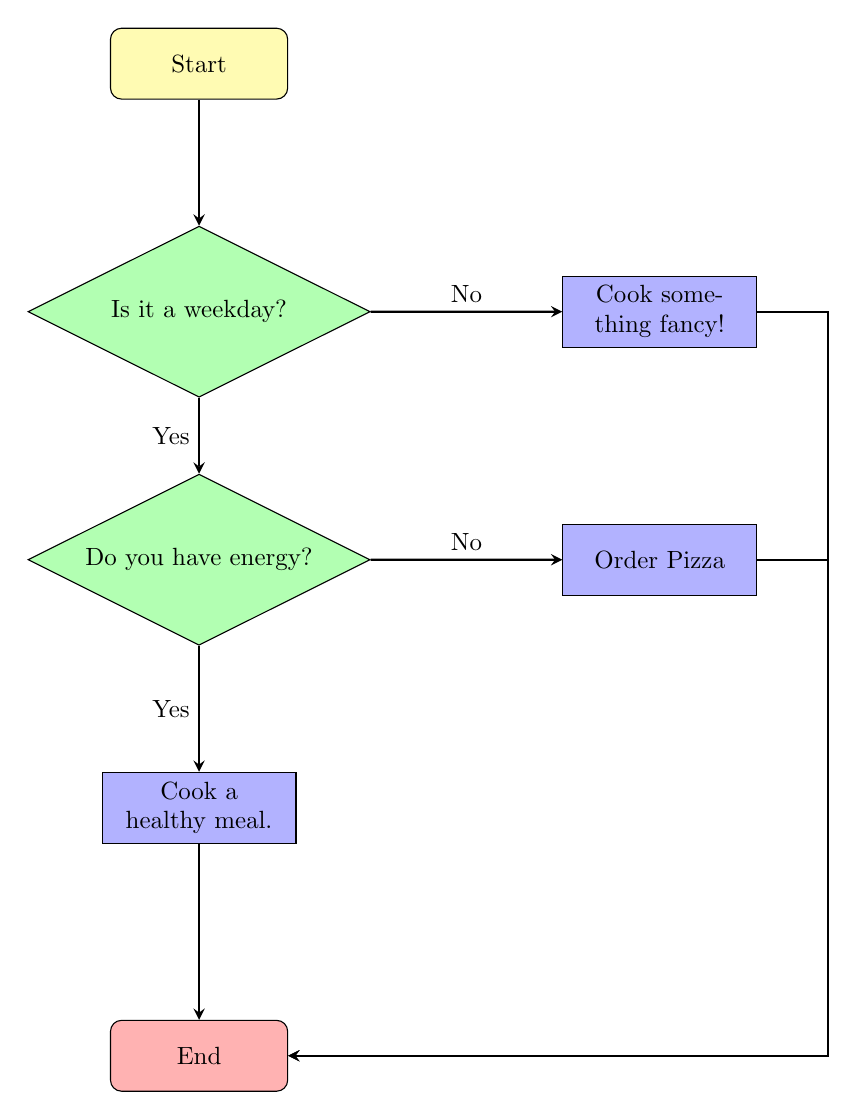
\begin{tikzpicture}[node distance=2.5cm, auto, scale=0.9, transform shape]
\node (start) [terminator, fill=yellow!30] {Start};
\node (dec1) [decision, below of=start, yshift=-1cm] {Is it a weekday?};
\node (proc1) [process, right of=dec1, xshift=4cm] {Cook something fancy!};
\node (dec2) [decision, below of=dec1, yshift=-1cm] {Do you have energy?};
\node (proc2) [process, right of=dec2, xshift=4cm] {Order Pizza};
\node (proc3) [process, below of=dec2, yshift=-1cm] {Cook a healthy meal.};
\node (end) [terminator, below of=proc3, yshift=-1cm] {End};

\draw [arrow] (start) -- (dec1);
\draw [arrow] (dec1) -- node[pos=0.5, above] {No} (proc1);
\draw [arrow] (dec1) -- node[pos=0.5, left] {Yes} (dec2);
\draw [arrow] (dec2) -- node[pos=0.5, above] {No} (proc2);
\draw [arrow] (dec2) -- node[pos=0.5, left] {Yes} (proc3);
\draw [arrow] (proc1.east) -- ++(1,0) |- (end);
\draw [arrow] (proc2.east) -- ++(1,0) |- (end);
\draw [arrow] (proc3) -- (end);
\end{tikzpicture}
\caption{The "Should I Get Takeaway?" Algorithm.}
\end{figure}

Look at that beautiful, logical flow. This isn't just a silly diagram; it's a perfect representation of an \texttt{if-else} statement.

\begin{lstlisting}[language=Python, caption={The flowchart, but in Python}]
# The flowchart, but in Python
is_weekday = True
have_energy = False

if is_weekday:
    if have_energy:
        print("Cook a healthy meal. You got this!")
    else:
        print("Order Pizza")
else:
    print("Cook something fancy!")
\end{lstlisting}

See? You just mapped a real-life decision directly to code. You thought in steps, and the code wrote itself.

\subsection{Example 2: The "Works on My Machine" Debugging Loop}

Now for something a little spicier. Every developer knows this pain. You write some code, it works perfectly, you ship it, and then... it explodes. Here's the universal debugging flowchart.

\begin{figure}[h!]
\centering
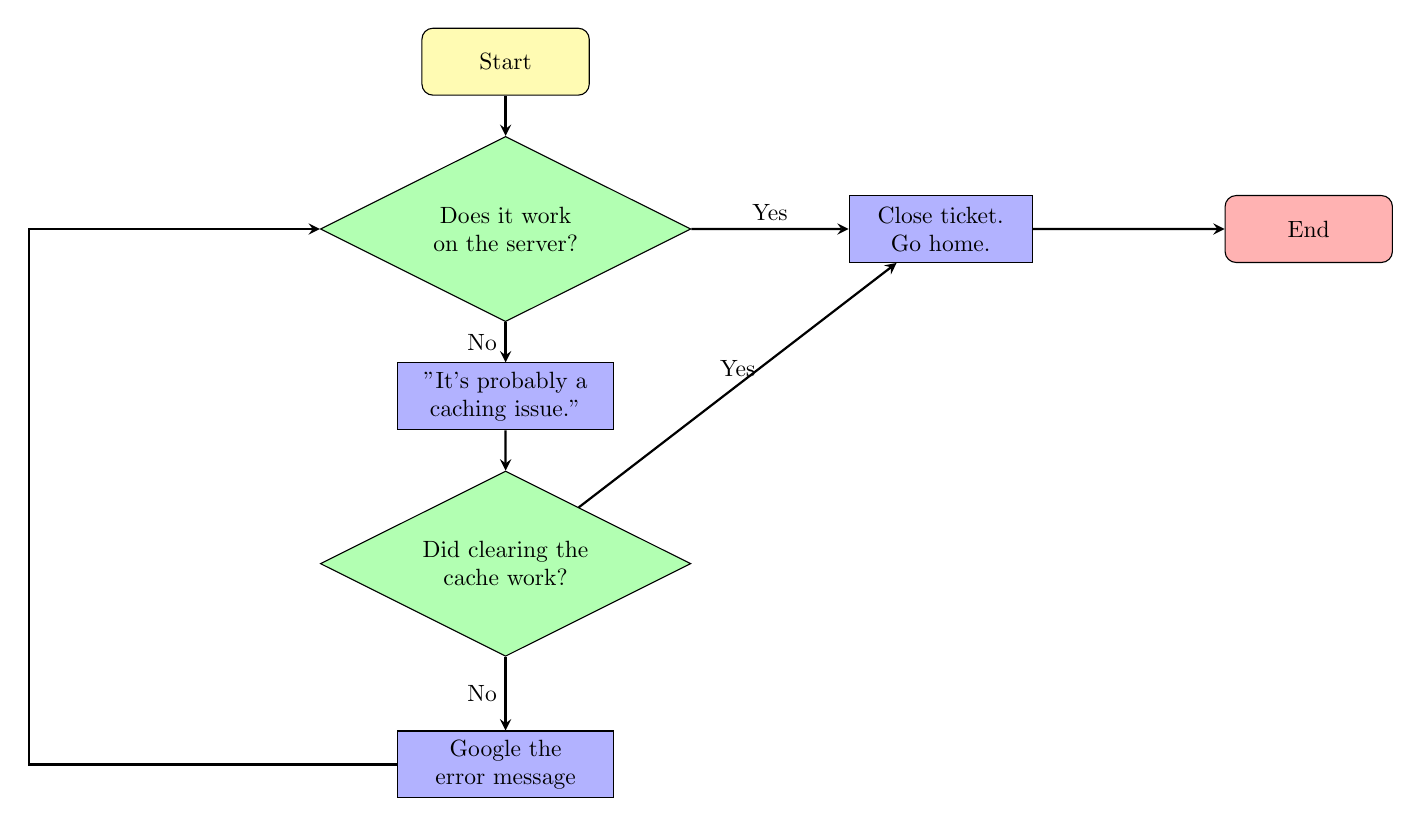
\begin{tikzpicture}[node distance=2cm, auto, scale=0.85, transform shape]
\node (start) [terminator, fill=yellow!30] {Start};
\node (dec1) [decision, below of=start, yshift=-0.5cm] {Does it work on the server?};
\node (proc1) [process, right of=dec1, xshift=4.5cm, text width=2.5cm] {Close ticket. Go home.};
\node (proc2) [process, below of=dec1, yshift=-0.5cm, text width=3cm] {"It's probably a caching issue."};
\node (dec2) [decision, below of=proc2, yshift=-0.5cm] {Did clearing the cache work?};
\node (proc3) [process, below of=dec2, yshift=-1cm, text width=3cm] {Google the error message};
\node (end) [terminator, right of=proc1, xshift=3.5cm] {End};

\draw [arrow] (start) -- (dec1);
\draw [arrow] (dec1) -- node[anchor=south] {Yes} (proc1);
\draw [arrow] (dec1) -- node[anchor=east] {No} (proc2);
\draw [arrow] (proc2) -- (dec2);
\draw [arrow] (dec2) -- node[anchor=south] {Yes} (proc1);
\draw [arrow] (dec2) -- node[anchor=east] {No} (proc3);
\draw [arrow] (proc1) -- (end);
% This creates the loop
\draw [arrow] (proc3.west) -| ++(-5.5,0) |- (dec1);
\end{tikzpicture}
\caption{The "Works on My Machine" Debugging Loop (Fixed).}
\end{figure}

This flowchart introduces a loop. We go from the Google step back to checking the server, repeating the process until the problem is solved. This is the essence of \texttt{while} loops and iterative problem-solving.

\section{From Funny to Functional: Why This Matters}

Okay, so we've had some fun with pizza and broken code. But here's the kicker: the logic you used to decide whether to say "hi" to that person you vaguely know from college is structurally identical to the logic a bank uses to flag a credit card transaction as fraudulent.

\textbf{"Should I say hi?" Flowchart:}
\begin{itemize}
    \item Do I know their name? $\rightarrow$ Yes
    \item Am I sure? $\rightarrow$ Yes
    \item Have we spoken in the last year? $\rightarrow$ No
    \item \textbf{Decision:} Awkwardly nod and walk faster.
\end{itemize}

\textbf{Fraud Detection Flowchart:}
\begin{itemize}
    \item Is the transaction amount > \$1000? $\rightarrow$ Yes
    \item Is the location unusual? $\rightarrow$ Yes
    \item Has the card been used in the last hour? $\rightarrow$ No
    \item \textbf{Decision:} Flag transaction and send a text alert.
\end{itemize}

Both are just a series of if-then-else checks. One prevents social awkwardness, the other prevents financial crime. The underlying logic is the same.

When we get to Chapter 6, you'll see that a Decision Tree is literally just a flowchart that an algorithm learns on its own. When we get to Chapter 10, you'll see that a Neural Network is just a much, much more complex flowchart with thousands of interconnected paths and decisions.

It all starts here. Learning to break problems down into these simple, visual steps is the most important skill you can develop. It's the foundation for everything that follows. Master the flowchart, and you've already taken your first giant leap into thinking like a machine learning engineer.

\begin{challengebox}
Your mission, should you choose to accept it:

Design a flowchart for the process of deciding whether to start working on a big, scary project.

Your flowchart must include:
\begin{itemize}
    \item At least two decision diamonds (e.g., "Is the deadline tomorrow?", "Is there coffee?").
    \item At least one loop (e.g., the classic "Watch one more YouTube video" loop).
    \item A "Panic Mode" process block.
\end{itemize}
Sketch it out on paper, use a tool, or even use ASCII art in a code comment.

\textbf{Bonus:} Translate your flowchart into a Python script with \texttt{if/else} statements and a \texttt{while} loop.

Don't just think about it. Draw it. It's the first step to rewiring your brain.
\end{challengebox}

% ===================================================================================
% CHAPTER 2
% ===================================================================================
\chapter{Math You Can’t Ignore (Sorry, Bestie)}

Okay, deep breaths. We need to talk about math.

I know, I know. You became a developer so you could build cool things, not relive your high school calculus nightmares. You just want to \texttt{import antigravity} and be done with it.

But here's the deal: machine learning isn't magic. It's math. You can't skip this chapter and expect to train a model that does anything other than set your CPU on fire. The good news? You don't need a PhD. You just need to understand three core concepts. We're going to treat this like ripping off a band-aid: quick, a little painful, but you'll feel so much better afterwards.

\section{Vectors \& Matrices: Spicy Python Lists}

Forget everything you think you know about vectors from physics class. In machine learning, a vector is just a fancy list of numbers that represents... well, anything.

\textbf{Analogy: The Fruit Stand}

Imagine you're at a fruit stand. You want to buy 2 apples, 3 bananas, and 4 clementines. You can represent your shopping list as a vector:
\[ \text{my\_stuff} = \begin{pmatrix} 2 \\ 3 \\ 4 \end{pmatrix} \]
The fruit stand has prices for each item: \$1 for an apple, \$2 for a banana, and \$3 for a clementine. We can represent this as a \texttt{prices} vector:
\[ \text{prices} = \begin{pmatrix} 1 \\ 2 \\ 3 \end{pmatrix} \]
Now, how do you calculate your total bill? You multiply the corresponding items and add them up:
\[ (2 \text{ apples} \times \$1/\text{apple}) + (3 \text{ bananas} \times \$2/\text{banana}) + (4 \text{ clementines} \times \$3/\text{clementine}) = \$2 + \$6 + \$12 = \$20 \]
Congratulations, you just did a \textbf{dot product}.

The dot product is how we "multiply" two vectors to get a single number. It's a measure of their interaction. In Python with NumPy, it's dead simple:

\begin{lstlisting}[language=Python]
import numpy as np

my_stuff = np.array([2, 3, 4])
prices = np.array([1, 2, 3])

# Calculate the dot product
total_bill = np.dot(my_stuff, prices)
print(f"Total bill: ${total_bill}") # Output: Total bill: $20
\end{lstlisting}

A \textbf{matrix} is just a stack of vectors. It's a spreadsheet. It's a list of lists. If you had shopping lists for three different people, you could stack them into a matrix:
\[ \text{all\_the\_stuff} = \begin{pmatrix} 2 & 3 & 4 \\ 1 & 1 & 5 \\ 3 & 2 & 0 \end{pmatrix} \begin{matrix} \leftarrow \text{My stuff} \\ \leftarrow \text{Friend 1's stuff} \\ \leftarrow \text{Friend 2's stuff} \end{matrix} \]
That's it. Vectors and matrices are just containers for our data. They're spicy arrays that let us do math on a whole bunch of numbers at once.

\section{Calculus: The Science of "How Fast Are We Screwing Up?"}

Calculus is all about change. For us, we care about one thing: finding the slope of a curve at a single point. This slope is called the \textbf{derivative}.

\textbf{Analogy: The Speedometer}

Imagine you're driving. Your total trip is 60 miles and it takes you an hour. Your average speed is 60 mph. Boring.

The derivative is your speedometer. It tells you your speed at this exact instant. Right now, you're going 75 mph. A second later, you hit traffic, and you're going 15 mph. The derivative is the instantaneous rate of change.

Why do we care? Because in machine learning, our "curve" is the \textbf{loss function} (which we'll cover in the next chapter). The loss function tells us how wrong our model is. The derivative of the loss function tells us the slope of our error.

\begin{figure}[h!]
\centering
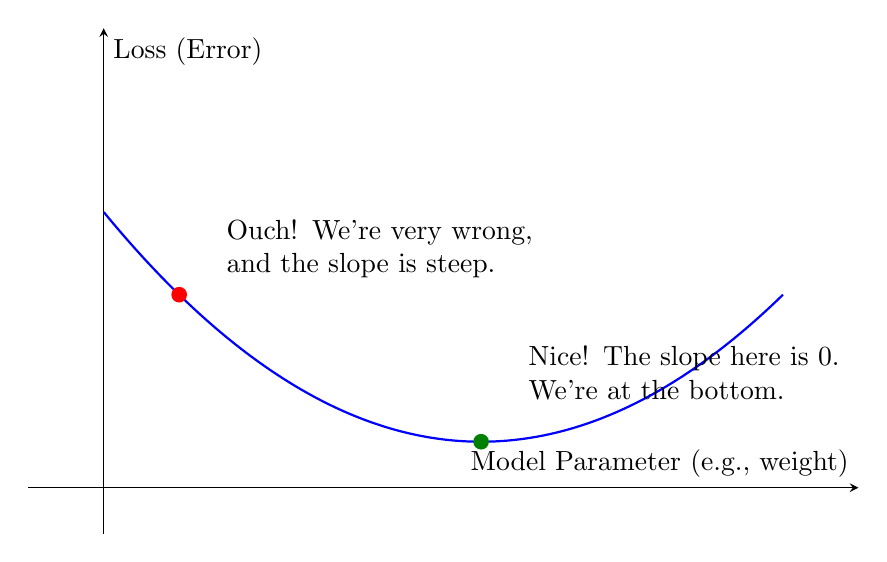
\begin{tikzpicture}
\begin{axis}[
    axis lines=middle,
    xlabel={Model Parameter (e.g., weight)},
    ylabel={Loss (Error)},
    xtick=\empty, ytick=\empty,
    xmin=-1, xmax=10,
    ymin=-1, ymax=10,
    width=\textwidth, % Make the plot responsive
    height=8cm,
    ]
    \addplot[domain=0:9, samples=100, smooth, thick, blue] {0.2*(x-5)^2 + 1};
    
    % Point on the steep part
    \node[circle, fill=red, inner sep=2pt] at (axis cs:1, 4.2) {};
    \node[anchor=west, text width=4cm] at (axis cs:1.5, 5.2) {Ouch! We're very wrong, and the slope is steep.};
    
    % Point at the minimum
    \node[circle, fill=green!50!black, inner sep=2pt] at (axis cs:5, 1) {};
    \node[anchor=west, align=left, text width=4cm] at (axis cs:5.5, 2.5) {Nice! The slope here is 0. We're at the bottom.};
\end{axis}
\end{tikzpicture}
\caption{Visualizing the loss curve and its derivative (Fixed).}
\end{figure}

The derivative tells us which way is "downhill" on our error curve. If the slope is negative, we need to increase our parameter to go down. If it's positive, we need to decrease it. If it's zero, we're at the bottom—we've found the minimum error! This process of following the derivative downhill is called \textbf{Gradient Descent}, and it's the engine of modern machine learning.

The joke goes: "The derivative of milk is cheese; the integral of milk is a cow". It's silly, but it captures the idea. The derivative breaks something down into its rate of change (milk -> cheese), while the integral builds it up (cow -> milk). We're in the cheese-making business.

\section{Probability: A Guided Tour of Your Gambling Addiction}

Probability is the language of uncertainty. And nowhere is uncertainty more expensive than in a casino.

\subsection{Expected Value: The House Always Wins}

Every casino game has a negative expected value for the player. This is the average amount you'd expect to win or lose per bet if you played forever.

Let's say you're playing a simple dice game. You bet \$1. If you roll a 6, you win \$5. If you roll anything else, you lose your \$1.
\begin{itemize}
    \item Probability of winning (rolling a 6) = 1/6
    \item Probability of losing (not rolling a 6) = 5/6
\end{itemize}
The expected value (EV) is calculated like this:
\[ \text{EV} = (P(\text{win}) \times \text{Amount won}) - (P(\text{lose}) \times \text{Amount lost}) \]
\[ \text{EV} = \left(\frac{1}{6} \times \$5\right) - \left(\frac{5}{6} \times \$1\right) = \frac{\$5}{6} - \frac{\$5}{6} = \$0 \]
Huh. This is a fair game. A casino would never offer this. Let's make it more realistic. They pay you \$4 if you win.
\[ \text{EV} = \left(\frac{1}{6} \times \$4\right) - \left(\frac{5}{6} \times \$1\right) = \frac{\$4}{6} - \frac{\$5}{6} = -\frac{\$1}{6} \approx -\$0.17 \]
This means that on average, every time you play, you lose 17 cents. This is the "house edge." A machine learning model's performance is similar. Over thousands of predictions, we want its average error—its expected loss—to be as close to zero as possible.

\subsection{Bayes' Theorem: Updating Your Beliefs}

Bayes' Theorem is a formal way to update your beliefs in the face of new evidence. Let's use a classic example: food allergies.

Let's say the probability that any random person has a peanut allergy is low, maybe 1\% ($P(\text{Allergy}) = 0.01$). This is our \textbf{prior belief}.

Now, your friend eats a cookie and their face swells up. This is \textbf{new evidence}. We want to calculate the probability they have an allergy \emph{given} this new evidence: $P(\text{Allergy} | \text{Swelling})$.

Bayes' Theorem gives us the formula:
\[ P(\text{Allergy} | \text{Swelling}) = \frac{P(\text{Swelling} | \text{Allergy}) \times P(\text{Allergy})}{P(\text{Swelling})} \]
This lets us update our initial 1\% belief to something much, much higher. This is exactly how the Naive Bayes algorithm (Chapter 8) works: it starts with a prior belief about the classes and updates that belief as it sees new data.

These three pillars—linear algebra for structure, calculus for optimization, and probability for uncertainty—are the bedrock of everything we're about to build. You survived. Now let's use them.

\begin{challengebox}
Time to put your new math skills to the test.
\begin{enumerate}
    \item \textbf{The House Edge:} A casino offers a game where you bet \$10 on a coin flip. Heads, you win \$9. Tails, you lose your \$10. The coin is fair (50/50 chance). Write a Python function to calculate the expected value of one bet. How much money does the casino expect to make off you per flip?
    \item \textbf{The High Roller:} A different game involves betting on three different outcomes with different payouts.
    \begin{itemize}
        \item Your bets are represented by a vector: \texttt{bets = [10, 0, 50]} (i.e., \$10 on game 1, \$0 on game 2, \$50 on game 3).
        \item The payout multipliers are a vector: \texttt{payouts = [1.2, 2.5, 0.8]}.
    \end{itemize}
    Use numpy to calculate your total winnings using a dot product. Did you make money or lose it?
\end{enumerate}
Show me the code!
\end{challengebox}

% ===================================================================================
% CHAPTER 3
% ===================================================================================
\chapter{The Algorithm is a Lazy Genius}

Alright, we've rewired our brains to think in flowcharts and we've stomached the necessary math. Now we get to the big question: what the hell is machine learning, really?

Forget the Skynet hype and the marketing buzzwords. Machine learning isn't magic. It's not sentient. It's more like a lazy but brilliant intern. This intern is incredibly good at finding patterns, but it only knows how to do two things:
\begin{enumerate}
    \item Check how badly it screwed up on a task.
    \item Take one tiny, incremental step to screw up a little less next time.
\end{enumerate}
That's it. That's the entire job description. The whole multi-billion dollar industry boils down to this simple, iterative loop. Let's break down the intern's workflow.

\section{Supervised vs. Unsupervised Learning: Clingy vs. Independent Algorithms}

First, we have to decide how we're going to manage our intern. There are two main management styles, and they define the two major branches of machine learning.

\subsection{Supervised Learning: The Micromanager's Dream}

This is learning with an answer key. You give the algorithm a ton of labeled data. For example, you give it 10,000 pictures of cats labeled "cat" and 10,000 pictures of dogs labeled "dog."

The intern's job is to learn the mapping from the input (the image) to the output (the label). It makes a guess ("I think this is a... cat?"), and you immediately tell it if it was right or wrong. It gets constant, direct feedback. It's "supervised."

\textbf{Analogy:} Studying for a test with a complete set of practice questions and the answer key.

\textbf{Examples:}
\begin{itemize}
    \item \textbf{Classification:} Is this email spam or not spam? (Discrete categories)
    \item \textbf{Regression:} How much will this house sell for? (Continuous value)
\end{itemize}

\subsection{Unsupervised Learning: The "Figure It Out Yourself" Approach}

This is learning without an answer key. You dump a massive pile of unlabeled data on the intern's desk and say, "Find something interesting." The algorithm has no idea what the "right" answers are. Its job is to find hidden patterns or structures in the data on its own.

\textbf{Analogy:} Being dropped in a new city without a map and told to find the "neighborhoods." You'd start grouping things by vibe: this area has lots of cafes (the 'hipster' cluster), this area has skyscrapers (the 'financial' cluster), etc.

\textbf{Examples:}
\begin{itemize}
    \item \textbf{Clustering:} Grouping customers into different market segments based on their purchasing habits.
    \item \textbf{Anomaly Detection:} Identifying fraudulent credit card transactions because they don't fit into any normal spending cluster.
\end{itemize}

Here's the cheat sheet:
\begin{table}[h!]
\centering
\begin{tabular}{|l|p{5cm}|p{5cm}|}
\hline
\textbf{Feature} & \textbf{Supervised Learning} & \textbf{Unsupervised Learning} \\
\hline
\textbf{Data} & Labeled (has an answer key) & Unlabeled (no answer key) \\
\hline
\textbf{Goal} & Predict a specific outcome & Discover hidden patterns/groups \\
\hline
\textbf{Analogy} & Student with a textbook \& answers & Explorer in a new land \\
\hline
\textbf{Common Tasks} & Regression, Classification & Clustering, Dimensionality Reduction \\
\hline
\textbf{Vibe} & Clingy, needs constant feedback & Independent, works it out alone \\
\hline
\end{tabular}
\caption{Supervised vs. Unsupervised Learning Cheat Sheet.}
\end{table}

For most of this book, we'll be focusing on supervised learning because it's easier to know if we're right or wrong.

\section{Training vs. Testing: Why Your Model Needs Boundaries}

This is one of the most critical concepts in all of ML, and it's where countless beginners trip up. You cannot evaluate your model's performance on the same data you used to train it. That's like giving a student the final exam questions to study with. Of course they'll get 100\%, but did they actually learn anything?

\textbf{Analogy: The Textbook and the Final Exam}

\begin{description}
    \item[Training Set:] This is the textbook, the lecture notes, and the homework problems. Your model can study this data as much as it wants. It sees both the questions (inputs) and the answers (labels). This is where it learns its parameters (the weights and biases). This is usually the largest chunk of your data, maybe 80\%.
    \item[Test Set:] This is the final, proctored exam. It contains questions the model has never seen before. The model only gets the inputs, makes its predictions, and we compare them to the answers which we've kept hidden. This gives us an unbiased measure of how well the model generalizes to new, unseen data. This is the true measure of success.
\end{description}

If you test your model on the training data, you're just measuring its ability to memorize, not its ability to learn. A model that gets 100\% on the training data but 50\% on the test data is a useless, over-caffeinated parrot.

\section{Loss Functions: "How Wrong Am I, on a Scale of 1 to 'Fire Me'?"}

So, our supervised intern makes a prediction. How do we give it feedback? We can't just say "you're wrong." We need to quantify \emph{how} wrong. That's the job of the \textbf{loss function} (also called a cost or error function).

\textbf{Analogy: The GPS Error}

A loss function is like a GPS telling you, "You are 500 feet from your destination." It's a single number that measures the distance between your model's prediction and the actual, ground-truth answer.

If the model predicts a house price of \$505,000 and the actual price was \$500,000, the loss might be \$5,000 (or some function of it).

If it predicts \$700,000, the loss will be much, much higher.

The goal of training is simple: \textbf{minimize the loss}. A small loss means your predictions are close to the truth. A large loss means your model is lost in the woods. The loss function provides the mathematical signal that tells our intern, "You screwed up by this much."

\section{Optimization: "How to Be Less Wrong, but Faster."}

Okay, the intern knows it screwed up by a value of, say, 14.7. Now what? It needs a strategy to be less wrong on the next try. This strategy is called an \textbf{optimizer}.

\textbf{Analogy: The Blindfolded Hiker}

Imagine our intern is blindfolded on a giant, hilly terrain. The altitude of the terrain is the loss. The goal is to get to the lowest point, the bottom of a valley.

How do you do it blindfolded?
\begin{enumerate}
    \item You feel the ground around your feet to find the direction of the steepest slope downwards. This "direction of steepest descent" is the \textbf{gradient} (which we get from the derivative of the loss function!).
    \item You take one small, careful step in that direction.
    \item You stop, feel the ground again, find the new steepest direction, and take another step.
\end{enumerate}
You repeat this over and over. Each step takes you a little bit lower. Eventually, you'll end up at the bottom of a valley.

This process is \textbf{Gradient Descent}, the most common optimizer in machine learning. It's the mechanism our lazy genius intern uses to iteratively adjust its internal parameters (weights) to minimize the loss.

This entire workflow—feeding in training data, making a prediction, calculating the loss, and using an optimizer to update the model—is the fundamental loop of supervised machine learning. It's not magic, it's just a lazy genius on a hill, taking one small step at a time.

\begin{challengebox}
Let's make this personal. Think about a skill you've learned, like cooking a new dish, playing a guitar chord, or even getting good at a video game.

Write out the "algorithm" for how you learned that skill, using the concepts from this chapter.

Identify the following:
\begin{itemize}
    \item What was your \textbf{training data}? (e.g., watching a recipe video, practicing scales)
    \item What was your \textbf{loss function}? How did you know you were wrong? (e.g., "The food is burnt," "The chord is buzzing," "I died again.")
    \item What was your \textbf{optimization step}? What tiny thing did you change for the next attempt? (e.g., "Lower the heat," "Press my finger down harder," "Don't run into that room.")
\end{itemize}
This exercise will prove to you that you're already an expert at this feedback loop. Now, we're just going to teach a computer to do it with code.
\end{challengebox}

% ===================================================================================
% PART 2
% ===================================================================================
\part{CORE MACHINE LEARNING – Real S\#!t Starts Here}

% ===================================================================================
% CHAPTER 4
% ===================================================================================
\chapter{DIY Linear Regression (a.k.a. Baby's First Model)}

Alright, buckle up. The theory is over. The hand-holding is done. It's time to write some code and build our very first model from scratch. No \texttt{sklearn}, no \texttt{Keras}, no magic black boxes. We're opening up the machine and building the engine ourselves with nothing but Python and NumPy.

Why? Because once you've built a car engine with your own hands, you'll never be afraid to look under the hood again.

Our mission is to build a \textbf{Linear Regression} model. It's the "Hello, World!" of machine learning. The goal is simple: predict a continuous value (like a house price or an exam score) by fitting a straight line to the data.

\section{The Goal: Predicting Stuff with a Straight Line}

Let's imagine a simple problem. We want to predict a student's final exam score based on the number of hours they studied. We have some data:

\begin{table}[h!]
\centering
\begin{tabular}{cc}
\hline
\textbf{Hours Studied (x)} & \textbf{Exam Score (y)} \\
\hline
2 & 65 \\
3 & 70 \\
5 & 75 \\
6 & 85 \\
8 & 90 \\
\hline
\end{tabular}
\end{table}

If we plot this, it looks something like this:

\begin{figure}[h!]
\centering
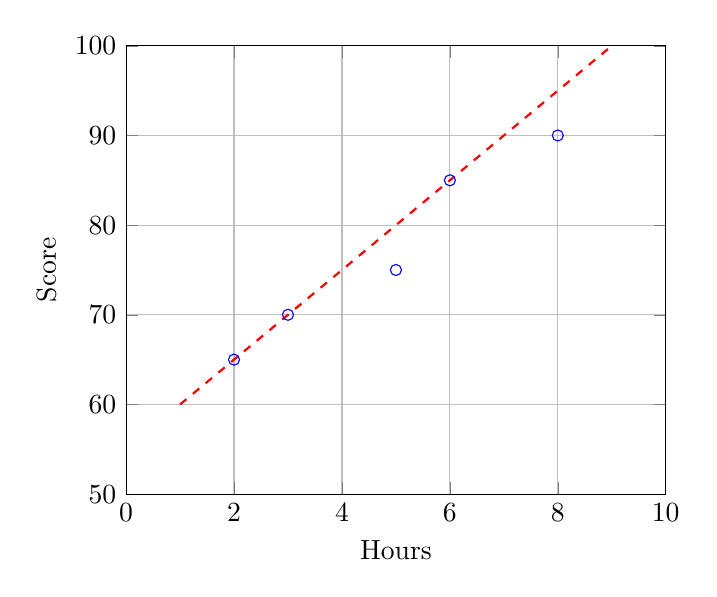
\begin{tikzpicture}
\begin{axis}[
    xlabel={Hours},
    ylabel={Score},
    xmin=0, xmax=10,
    ymin=50, ymax=100,
    grid=major,
    ]
    \addplot[only marks, mark=o, blue] table {
        x y
        2 65
        3 70
        5 75
        6 85
        8 90
    };
    \addplot[domain=1:9, red, thick, dashed] {5*x + 55};
\end{axis}
\end{tikzpicture}
\caption{Exam score vs. hours studied.}
\end{figure}

You can see a clear trend: more hours studied generally leads to a higher score. A straight line seems like a reasonable way to model this relationship. And what's the equation for a straight line? You know this from middle school.
\[ y = mx + b \]
\begin{itemize}
    \item \textbf{y:} The value we want to predict (Exam Score).
    \item \textbf{x:} Our input feature (Hours Studied).
    \item \textbf{m:} The slope of the line. How much the score increases for each extra hour of study.
    \item \textbf{b:} The y-intercept (or bias). The score someone would get with 0 hours of study (maybe they're just a genius).
\end{itemize}
In machine learning, we often call \textbf{m} the \textbf{weight} and \textbf{b} the \textbf{bias}. The "learning" part of linear regression is just finding the best possible values for \textbf{m} and \textbf{b} that make our line fit the data as closely as possible.

\section{Code-First Implementation: Let's Get Our Hands Dirty}

Let's fire up our editor and build this thing piece by piece.

\subsection{Step 1: The \texttt{predict()} Function}

First, we need a function that, given an input \texttt{x} and our line's parameters \texttt{m} and \texttt{b}, can predict what \texttt{y} should be. This is just the line equation.

\begin{lstlisting}[language=Python]
import numpy as np

# Let's start with some random guesses for our parameters
m = 0.5
b = 20

# Our data
X = np.array([2, 3, 5, 6, 8])
y_true = np.array([65, 70, 75, 85, 90])

def predict(X, m, b):
    # This is literally just y = mx + b
    # We use X (capital) because in ML, our inputs are usually a matrix
    return m * X + b

# Let's see our initial, terrible predictions
y_pred = predict(X, m, b)
print(y_pred)
# Output: [21.  21.5 22.5 23.  24. ] -> Yeah, our model sucks right now.
\end{lstlisting}

\subsection{Step 2: The \texttt{loss()} Function (Mean Squared Error)}

Our model is terrible. But how terrible? We need to quantify the error. We'll use the most common loss function for regression: \textbf{Mean Squared Error (MSE)}.

The logic is simple:
\begin{enumerate}
    \item For each data point, calculate the difference between the true score (\texttt{y\_true}) and our predicted score (\texttt{y\_pred}). This is the \textbf{error}.
    \item \textbf{Square} the error. This does two things: it makes all errors positive, and it punishes big errors way more than small ones. An error of 4 becomes 16, while an error of 2 only becomes 4.
    \item Calculate the \textbf{average} of all these squared errors.
\end{enumerate}
\[ \text{MSE} = \frac{1}{n} \sum_{i=1}^{n} (y_{\text{true}, i} - y_{\text{pred}, i})^2 \]

\begin{lstlisting}[language=Python]
def loss(y_true, y_pred):
    # This is the Mean Squared Error formula
    return np.mean((y_true - y_pred)**2)

# Let's calculate our initial loss
initial_loss = loss(y_true, y_pred)
print(f"Initial Loss: {initial_loss}")
# Output: Initial Loss: 4044.85 -> Ouch. That's a big number. We need to lower it.
\end{lstlisting}

\subsection{Step 3: The \texttt{update()} Function (Gradient Descent)}

This is the heart of the machine. How do we find better values for \texttt{m} and \texttt{b}? We use the "blindfolded hiker" method: Gradient Descent.

We need to calculate the gradient of our loss function. The gradient is just a vector of partial derivatives—one for \texttt{m} and one for \texttt{b}. These derivatives tell us the slope of the loss with respect to each parameter.

Don't worry, I'll spare you the full calculus derivation. The partial derivatives of our MSE loss function are:
\begin{itemize}
    \item Derivative with respect to m ($\frac{\partial L}{\partial m}$): $-2 \times \text{mean}(X \times (y_{\text{true}} - y_{\text{pred}}))$
    \item Derivative with respect to b ($\frac{\partial L}{\partial b}$): $-2 \times \text{mean}(y_{\text{true}} - y_{\text{pred}})$
\end{itemize}
These formulas tell us which way is "downhill" for \texttt{m} and \texttt{b}. To descend the hill, we just need to take a small step in the \emph{opposite} direction of the gradient.

\begin{lstlisting}[language=Python]
# We need a learning rate. This is the size of the step we take.
# It's a "hyperparameter" - a knob we have to tune.
learning_rate = 0.01

def update(X, y_true, y_pred, m, b, learning_rate):
    # Calculate the gradients
    dm = -2 * np.mean(X * (y_true - y_pred))
    db = -2 * np.mean(y_true - y_pred)

    # Update the parameters by taking a small step downhill
    new_m = m - learning_rate * dm
    new_b = b - learning_rate * db
    return new_m, new_b
\end{lstlisting}

\section{Putting It All Together: The Training Loop}
Now we just need to put these pieces into a loop. We'll repeat the process of predicting, calculating loss, and updating our parameters for a set number of times (called \textbf{epochs}).

\begin{lstlisting}[language=Python]
# Let's reset our parameters and start training
m = 0.0
b = 0.0
epochs = 1000
learning_rate = 0.01

loss_history = [] # To store our loss at each step

for i in range(epochs):
    # 1. Make predictions
    y_pred = predict(X, m, b)

    # 2. Calculate loss
    current_loss = loss(y_true, y_pred)
    loss_history.append(current_loss)

    # Print the loss every 100 epochs to see our progress
    if i % 100 == 0:
        print(f"Epoch {i}: Loss = {current_loss:.2f}, m = {m:.2f}, b = {b:.2f}")

    # 3. Update the parameters
    m, b = update(X, y_true, y_pred, m, b, learning_rate)

print("\n--- Training Complete ---")
print(f"Final Loss: {loss_history[-1]:.2f}")
print(f"Optimal parameters: m = {m:.2f}, b = {b:.2f}")
\end{lstlisting}

If you run this, you'll see the loss steadily decreasing. It's learning!

\section{Visualizing the Heartbeat}
The most satisfying part is watching the loss curve. It's like a heartbeat monitor for your model's learning process.

\begin{lstlisting}[language=Python]
import matplotlib.pyplot as plt

plt.plot(loss_history)
plt.title("Loss Curve During Training")
plt.xlabel("Epoch")
plt.ylabel("Mean Squared Error")
plt.show()
\end{lstlisting}

\begin{figure}[h!]
\centering
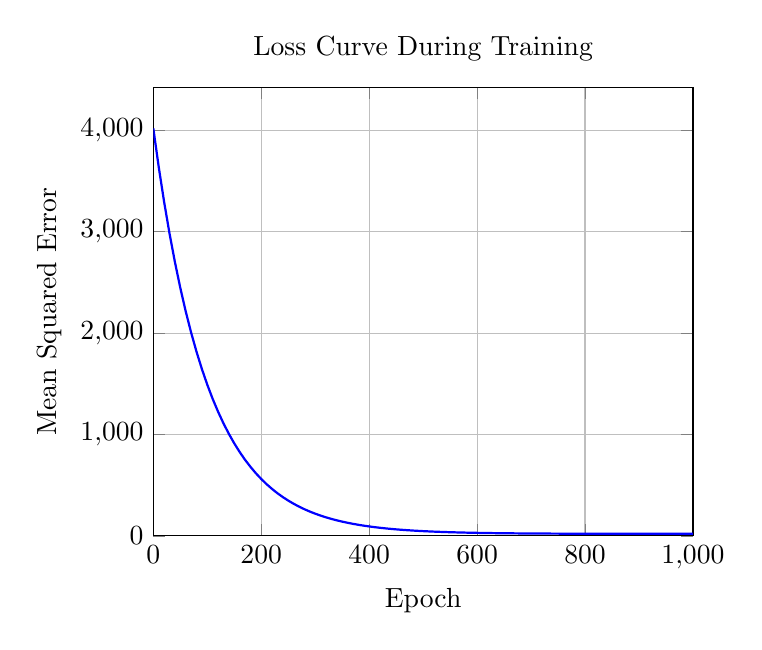
\begin{tikzpicture}
\begin{axis}[
    title={Loss Curve During Training},
    xlabel={Epoch},
    ylabel={Mean Squared Error},
    xmin=0, xmax=1000,
    ymin=0,
    grid=major,
    ]
    \addplot[domain=0:1000, samples=101, blue, thick, no marks] {4000*exp(-x/100)+20};
\end{axis}
\end{tikzpicture}
\caption{A typical loss curve for linear regression training.}
\end{figure}

You should see a beautiful curve that drops steeply at first and then flattens out as the model converges on the best possible \texttt{m} and \texttt{b}.

This is it. This \texttt{predict -> loss -> update} loop is the fundamental engine of nearly all supervised learning, from this simple line-fitter to massive neural networks like GPT. The models get more complex, the \texttt{predict} function becomes a monstrous beast, and the \texttt{update} step uses more advanced calculus (hello, backpropagation), but the core logic you just built remains the same. You didn't just build a linear regression model. You built the blueprint.

\begin{challengebox}
You've built a working model. Now it's time to break it.
Take the training loop code we just wrote.
Run it three times with three different \texttt{learning\_rate} values:
\begin{itemize}
    \item A "good" one: 0.01
    \item A "too low" one: 0.0001
    \item A "too high" one: 0.1
\end{itemize}
For each run, plot the \texttt{loss\_history}.

Analyze the results:
\begin{itemize}
    \item What happens to the loss curve when the learning rate is too low?
    \item What happens when it's too high? (You might see \texttt{NaN} or ridiculously large numbers. This is called \textbf{divergence}, and it's hilarious.)
    \item Explain why this happens, using the "blindfolded hiker" analogy.
\end{itemize}
This is your first taste of a critical ML skill: \textbf{hyperparameter tuning}. Welcome to the club.
\end{challengebox}

\chapter{Classification: The “Yes or No” Saga}
\label{chap:classification}

Great, you've taught a machine to draw a straight line. Impressive. You can now predict house prices, exam scores, and other things that live on a continuous number line.

But what about the questions that really matter?
\begin{itemize}
    \item Is this email spam? (Yes/No)
    \item Is this credit card transaction fraudulent? (Yes/No)
    \item Is this a picture of a hot dog? (Hot Dog/Not Hot Dog)
\end{itemize}
These are classification problems. We don't want a number; we want a decision. A simple "yes" or "no." Let's teach our model how to make a choice.

\section{Why Linear Regression Fails for Classification}

Your first instinct might be to just use the linear regression model we just built. Let's say "No" is class 0 and "Yes" is class 1. Why can't we just fit a line to that?

Let's try it. Imagine we're predicting whether a tumor is malignant (1) or benign (0) based on its size.

\begin{figure}[h!]
\centering
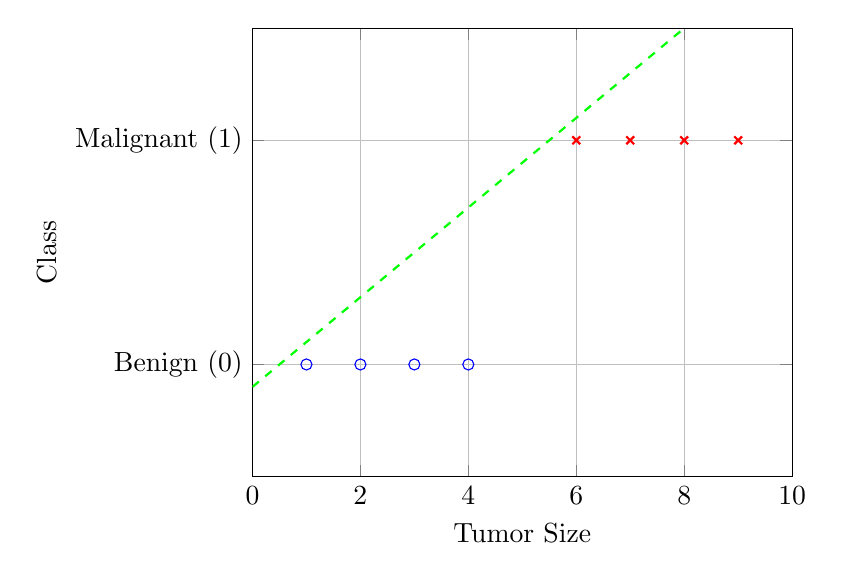
\begin{tikzpicture}
\begin{axis}[
    xlabel={Tumor Size},
    ylabel={Class},
    xmin=0, xmax=10,
    ymin=-0.5, ymax=1.5,
    ytick={0,1},
    yticklabels={Benign (0), Malignant (1)},
    grid=major,
    ]
    % Benign points
    \addplot[only marks, mark=o, blue] table {
        x y
        1 0
        2 0
        3 0
        4 0
    };
    % Malignant points
    \addplot[only marks, mark=x, red, thick] table {
        x y
        6 1
        7 1
        8 1
        9 1
    };
    % Bad linear regression fit
    \addplot[domain=0:10, green, thick, dashed] {0.2*x - 0.1};
\end{axis}
\end{tikzpicture}
\caption{Linear regression is a poor fit for classification.}
\end{figure}

See the problem? Our beautiful line shoots off to infinity in both directions. It can predict a value of 1.8, or -0.4. What does a "malignancy probability" of 180\% even mean? Or -40\%? It's nonsense. It breaks our 0-or-1 world.

We need a new tool. We need something that takes the output of our linear equation and squishes it into a sensible range: between 0 and 1.

\section{Enter the Sigmoid Function: The OG 'Squishinator'}

Meet your new best friend: the \textbf{Sigmoid function}. It's a beautiful, elegant, S-shaped curve that is the absolute hero of binary classification.

The formula is:
\[ \sigma(z) = \frac{1}{1 + e^{-z}} \]
Where $z$ is just the output of our old friend, the linear equation: $z = mx + b$.

Here's what it looks like and why it's so perfect:

\begin{figure}[h!]
\centering
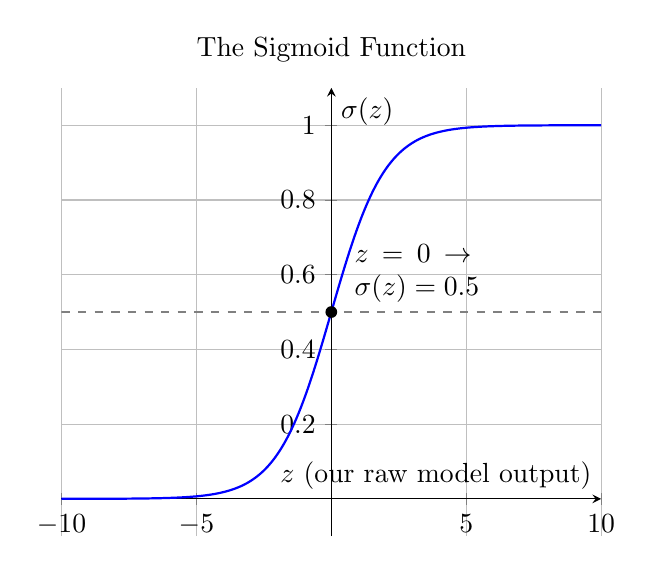
\begin{tikzpicture}
\begin{axis}[
    title={The Sigmoid Function},
    xlabel={$z$ (our raw model output)},
    xlabel style={yshift=0.5em}, % Lift the label to prevent cutoff
    ylabel={$\sigma(z)$},
    xmin=-10, xmax=10,
    ymin=-0.1, ymax=1.1, % Add padding to avoid cutoff
    grid=major,
    axis lines=middle,
    ]
    \addplot[domain=-10:10, samples=100, smooth, thick, blue] {1/(1+exp(-x))};
    \addplot[dashed, gray] coordinates {(-10, 0.5) (10, 0.5)};
    \node[circle,fill,inner sep=1.5pt] at (axis cs:0,0.5) {};
    \node[above right, text width=2cm] at (axis cs:0.5, 0.5) {$z=0 \rightarrow \sigma(z)=0.5$};
\end{axis}
\end{tikzpicture}
\caption{The elegant S-curve of the Sigmoid function.}
\end{figure}

Look at its properties:
\begin{itemize}
    \item It takes any real number, from negative infinity to positive infinity.
    \item It squishes that number into a range between 0 and 1.
    \item A very large positive input for $z$ gets mapped close to 1.
    \item A very large negative input for $z$ gets mapped close to 0.
    \item An input of $z=0$ gets mapped to exactly 0.5.
\end{itemize}
This is exactly what we need! We can now interpret the output of the sigmoid function as a \textbf{probability}.
\begin{itemize}
    \item If our model outputs 0.98, it's 98\% sure the answer is "Yes" (Class 1).
    \item If it outputs 0.05, it's 95\% sure the answer is "No" (or 5\% sure it's "Yes").
    \item If it outputs 0.5, it's completely uncertain. Flip a coin.
\end{itemize}
The sigmoid is like a translator that turns the raw, unbounded "score" from our linear model into a calibrated, understandable probability.

\section{DIY Logistic Regression: It's a Trap!}

Now we're going to build a \textbf{Logistic Regression} model from scratch. And here's the secret that confuses everyone: despite its name, Logistic Regression is for \textbf{CLASSIFICATION}, not regression. The name is a historical accident designed to trip up beginners. Don't fall for it.

You're about to have a "wait a minute..." moment, because the code is going to look suspiciously familiar.

\subsection{Step 1: The \texttt{predict()} function}

This is almost the same as before, but we just wrap our linear equation in our new sigmoid function.

\begin{lstlisting}[language=Python]
import numpy as np

def sigmoid(z):
    return 1 / (1 + np.exp(-z))

def predict_proba(X, m, b):
    # Same linear equation as before
    z = m * X + b
    # But now we squish the result!
    return sigmoid(z)
\end{lstlisting}

\subsection{Step 2: The \texttt{loss()} function (Binary Cross-Entropy)}

We can't use Mean Squared Error anymore. For classification, we need a loss function that punishes the model when it's confidently wrong. We use \textbf{Binary Cross-Entropy} (or Log Loss).

The formula looks scary, but the intuition is simple:
\[ \text{Loss} = -\frac{1}{n} \sum_{i=1}^{n} [y_i \log(\hat{y}_i) + (1-y_i) \log(1-\hat{y}_i)] \]
\begin{itemize}
    \item If the true label is 1 ($y_i=1$), the loss is $-\log(\hat{y}_i)$. If our model predicts 0.99 (close to 1), the log is close to 0, so the loss is small. If it predicts 0.01 (confidently wrong), the log is a large negative number, so the loss is huge.
    \item If the true label is 0 ($y_i=0$), the loss is $-\log(1-\hat{y}_i)$. The same logic applies in reverse.
\end{itemize}

\begin{lstlisting}[language=Python]
def loss(y_true, y_pred):
    # Binary Cross-Entropy
    # We add a small epsilon to prevent log(0) errors
    epsilon = 1e-15
    y_pred = np.clip(y_pred, epsilon, 1 - epsilon)
    return -np.mean(y_true * np.log(y_pred) + (1 - y_true) * np.log(1 - y_pred))
\end{lstlisting}

This loss function brutally punishes the model for being cocky and wrong, which is exactly what we want.

\subsection{Step 3: The \texttt{update()} function (Still Gradient Descent!)}

Guess what? The update mechanism is still Gradient Descent. The derivative of the Binary Cross-Entropy loss with respect to our parameters \texttt{m} and \texttt{b} turns out to be surprisingly simple.
\begin{itemize}
    \item Derivative with respect to m ($\frac{\partial L}{\partial m}$): $\text{mean}((\hat{y} - y) \times X)$
    \item Derivative with respect to b ($\frac{\partial L}{\partial b}$): $\text{mean}(\hat{y} - y)$
\end{itemize}
The update loop looks identical to the one in linear regression. We just swapped out the engine parts (\texttt{predict} and \texttt{loss} functions), but the chassis is the same.

This reveals a fundamental concept in ML: algorithms are often just clever combinations of simpler pieces. We didn't learn a totally new algorithm; we learned a "plugin" (the sigmoid function and a new loss) that adapted our linear model for a new task.

\section{Decision Boundaries: Drawing the Line (Literally)}

So what does our trained logistic regression model actually do? It learns a \textbf{decision boundary}. For a 2D problem, this is a line.

\begin{figure}[h!]
\centering
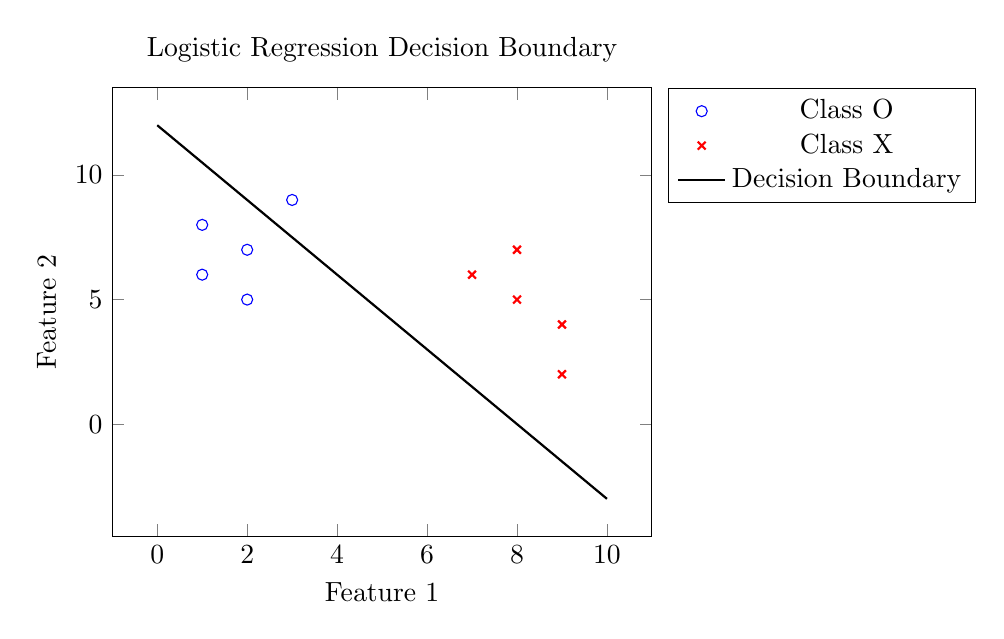
\begin{tikzpicture}
\begin{axis}[
    title={Logistic Regression Decision Boundary},
    xlabel={Feature 1},
    ylabel={Feature 2},
    legend pos=outer north east,
    ]
    % Class O
    \addplot[only marks, mark=o, blue] table {
        x y
        1 8
        2 7
        1 6
        3 9
        2 5
    };
    \addlegendentry{Class O}
    
    % Class X
    \addplot[only marks, mark=x, red, thick] table {
        x y
        7 6
        8 5
        9 4
        8 7
        9 2
    };
    \addlegendentry{Class X}
    
    % Decision Boundary
    \addplot[domain=0:10, black, thick] {-1.5*x + 12};
    \addlegendentry{Decision Boundary}
\end{axis}
\end{tikzpicture}
\caption{A linear decision boundary separating two classes.}
\end{figure}

The model has learned a line that best separates the 'O's from the 'X's. Any new point that falls on one side of the line is classified as 'X', and any point on the other is classified as 'O'. This is how the model makes its decision. It's not just predicting probabilities; it's literally drawing a line in the sand.

\begin{challengebox}
The XOR Problem

You've built a powerful classifier. It can separate data with a straight line. But what happens when a straight line isn't enough?

Create the classic XOR dataset:
\begin{itemize}
    \item Inputs: \texttt{[[0, 0], [0, 1], [1, 0], [1, 1]]}
    \item Outputs: \texttt{[0, 1, 1, 0]}
\end{itemize}
Try to train your from-scratch Logistic Regression model on this data.

Plot the loss curve. What happens? Does it converge?

Explain why it fails. Can you draw a single straight line that can separate the XOR data points if you plot them?

This failure is not a bug in your code. It's a fundamental limitation of linear models. And it's the perfect motivation for why we're going to need something much more powerful: Neural Networks.
\end{challengebox}

\chapter{Decision Trees: The Judgmental Algorithm}

So far, the models we've built have been a bit... abstract. They find the best-fit line or the best-separating plane by fiddling with weights and biases. They give us an answer, but the reasoning is hidden inside a mathematical formula.

Now, let's build a model you can argue with. A model that's as transparent as it is judgmental.

Meet the \textbf{Decision Tree}.

Imagine an algorithm that makes decisions like a paranoid, hyper-specific auntie asking 20 questions before letting you borrow her car. "Is the weather nice? Are you going on the highway? Did you check the tire pressure? Is your friend Chad going with you? I don't like Chad."

That's a Decision Tree. It's basically a flowchart on steroids, and it's one of the most intuitive and interpretable models in all of machine learning.

\section{A Flowchart That Learns}

Remember Chapter 1? We said a Decision Tree is just a flowchart that an algorithm learns from data. That's literally it.

\begin{figure}[h!]
\centering
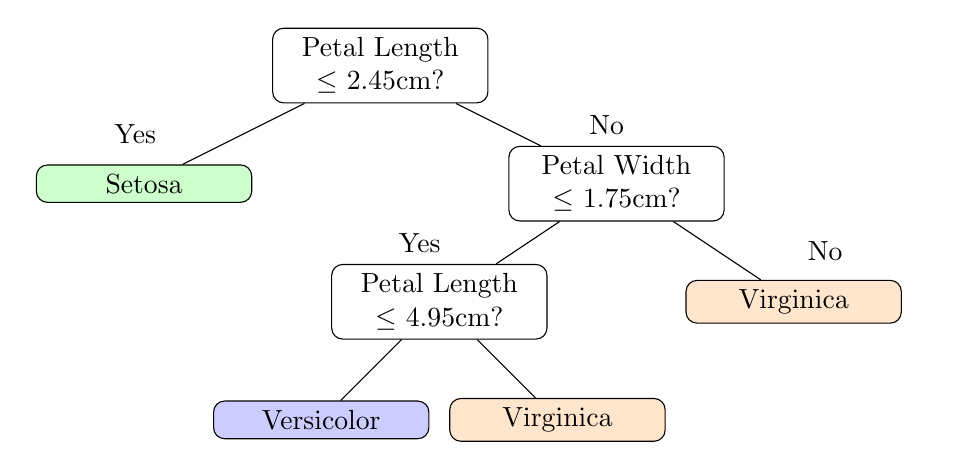
\begin{tikzpicture}[
    level 1/.style={sibling distance=6cm},
    level 2/.style={sibling distance=4.5cm},
    level 3/.style={sibling distance=3cm},
    every node/.style={draw, rectangle, rounded corners, align=center, text width=2.5cm}
]
\node {Petal Length $\le$ 2.45cm?}
    child {node[fill=green!20] {Setosa} edge from parent node[left, draw=none] {Yes}}
    child {node {Petal Width $\le$ 1.75cm?}
        child {node {Petal Length $\le$ 4.95cm?}
            child {node[fill=blue!20] {Versicolor}}
            child {node[fill=orange!20] {Virginica}}
        edge from parent node[left, draw=none] {Yes}}
        child {node[fill=orange!20] {Virginica} edge from parent node[right, draw=none] {No}}
    edge from parent node[right, draw=none] {No}};
\end{tikzpicture}
\caption{A simple decision tree for classifying Iris flowers.}
\end{figure}

Each internal node is a question about a feature (e.g., "Is age < 30?").
Each branch is an answer to that question (e.g., "Yes" or "No").
Each leaf node is a final decision or prediction (e.g., "Class = 'Buys the Product'").

The genius of the algorithm is that it figures out the best questions to ask, and in what order, to make the most accurate predictions.

\section{The Big Question: What's the Best Question?}

How does the tree decide to ask "Is age < 30?" instead of "Is income > \$50k?" It needs a way to measure how "good" a question is. A good question is one that splits a mixed group of data into purer, more organized subgroups.

We measure this purity (or lack thereof) with metrics like \textbf{Gini Impurity} or \textbf{Entropy}.

\textbf{Analogy: The Fruit Basket of Chaos}

Imagine you have a basket of 10 fruits.
\begin{itemize}
    \item \textbf{Scenario 1: Perfect Purity.} The basket has 10 apples. If you reach in, you're 100\% certain you'll grab an apple. The chaos is zero.
    \begin{itemize}
        \item Gini Impurity = 0
        \item Entropy = 0
    \end{itemize}
    \item \textbf{Scenario 2: Maximum Impurity.} The basket has 5 apples and 5 oranges. It's a 50/50 shot. The chaos is at its maximum. You have no idea what you'll get.
    \begin{itemize}
        \item Gini Impurity = 0.5 (for a two-class problem)
        \item Entropy = 1.0
    \end{itemize}
\end{itemize}

The Decision Tree algorithm works by trying out every possible split on every feature. For each split, it calculates the impurity of the resulting child nodes. It then chooses the split that results in the biggest decrease in impurity. This decrease is called \textbf{Information Gain}. The tree is greedy; it always picks the split that gives it the most information right now.

\begin{description}
    \item[Gini Impurity:] The probability of incorrectly classifying a randomly chosen element if it were randomly labeled according to the distribution of labels in the subset. It's computationally faster than Entropy because it doesn't involve a logarithm. The formula is $G = 1 - \sum_{i=1}^{C} (p_i)^2$.
    \item[Entropy:] A concept from information theory measuring the level of uncertainty or randomness. The formula is $H = -\sum_{i=1}^{C} p_i \log_2(p_i)$.
\end{description}

In practice, they both do a very similar job. Gini is the default for many libraries (like scikit-learn's CART algorithm) because it's a bit quicker to compute.

\section{From-Scratch Implementation: Building the Tree Recursively}

Building a decision tree is a classic example of a recursive algorithm.

\begin{description}
    \item[\texttt{find\_best\_split()}:] This is the workhorse function. It needs to:
    \begin{enumerate}
        \item Loop through every column (feature) in the data.
        \item Loop through every unique value in that column (as a potential split point).
        \item For each potential split, divide the data into two groups (left and right).
        \item Calculate the Gini Impurity of the split (a weighted average of the impurity of the two child nodes).
        \item Keep track of the split that produced the lowest Gini Impurity so far.
    \end{enumerate}
    Return the best feature and split value.
    \item[\texttt{build\_tree()}:] This is the recursive function.
    \begin{itemize}
        \item It takes a dataset (a node) as input.
        \item It calls \texttt{find\_best\_split()} on that data.
        \item \textbf{Base Case (Stopping Condition):} If a stopping condition is met, it becomes a leaf node and returns a prediction (e.g., the majority class of the data points at that node). Stopping conditions could be:
        \begin{itemize}
            \item The node is perfectly pure (Gini = 0).
            \item The tree has reached a \texttt{max\_depth} we defined.
            \item The number of samples in the node is below a \texttt{min\_samples\_leaf} threshold.
        \end{itemize}
        \item \textbf{Recursive Step:} If no stopping condition is met, it creates a new internal node based on the best split. It then calls \texttt{build\_tree()} on the left group and the right group, assigning the results to the left and right branches of the current node.
    \end{itemize}
\end{description}

\begin{lstlisting}[language=Python, caption={Super simplified pseudo-code}]
def build_tree(data):
    # Check for stopping conditions (base cases)
    if is_pure(data) or reached_max_depth(data):
        return create_leaf_node(data) # Return the majority class

    # Find the best question to ask
    best_feature, best_value = find_best_split(data)
    
    # Split the data based on the question
    left_data, right_data = split(data, best_feature, best_value)

    # Recursively build the sub-trees
    left_subtree = build_tree(left_data)
    right_subtree = build_tree(right_data)

    # Return the node representing this question and its branches
    return Node(question=(best_feature, best_value), 
                left_branch=left_subtree, 
                right_branch=right_subtree)
\end{lstlisting}

\section{Overfitting: When the Tree Becomes a Forest Fire}

What happens if you don't set any stopping conditions? The tree will keep splitting and splitting until every single leaf node is perfectly pure. It might even create a leaf node for a single, noisy data point.

This is \textbf{overfitting}, and decision trees are notoriously prone to it.

\textbf{Analogy: The Over-Specific Student}

Imagine a student studying for a history exam.
\begin{itemize}
    \item A \textbf{good student} learns the general patterns: "Revolutions are often caused by economic inequality and new political ideas."
    \item An \textbf{overfit student} memorizes hyper-specific, useless facts: "On October 5th, 1789, a man named Dave in Paris complained about the price of bread while wearing a blue hat."
\end{itemize}
The overfit student gets 100\% on the practice questions that cover Dave, but when the real exam asks a general question about the causes of the French Revolution, they have no idea what to say.

An overfit decision tree is the same. It learns the noise and quirks of the training data perfectly, resulting in a ridiculously complex tree that looks like a spider web. It performs great on the data it has seen, but it fails spectacularly on new, unseen data.

The solution is \textbf{pruning}. This can be:
\begin{itemize}
    \item \textbf{Pre-pruning (Early Stopping):} Don't let the tree grow too deep in the first place. This is what our \texttt{max\_depth} and \texttt{min\_samples\_leaf} hyperparameters do.
    \item \textbf{Post-pruning:} Grow the full tree first, then go back and remove branches that don't provide much information gain.
\end{itemize}

By limiting the tree's complexity, we force it to learn the general patterns, not the noise. This is a crucial step in building a tree that actually works in the real world. The tree's greatest strength—its ability to create specific rules—is also its greatest weakness. Its interpretability is a direct window into its fragility; a small change in the input data can lead to a completely different set of learned rules. This sensitivity is exactly why more robust methods, like Random Forests (which we'll hint at later), were invented—they build an entire committee of these unstable trees and let them vote, turning a collection of shaky experts into a wise crowd.

\begin{challengebox}
Visualize Your Judgment

You've built a tree from scratch. Now let's make it talk.

Write a \texttt{print\_tree()} function that takes your trained tree (the root node) and prints out the rules in a human-readable, indented format.

Example output:
\begin{verbatim}
if (petal_width_cm <= 0.8):
--> predicts: setosa
else:
--> if (petal_length_cm <= 4.95):
    --> predicts: versicolor
    --> else:
        --> predicts: virginica
\end{verbatim}

Train your tree on a simple, classic dataset like the Iris dataset.

Use your new function to print the learned rules. Do they make intuitive sense? Can you follow the logic from the root to a leaf?

This is the superpower of decision trees. You're not just getting a prediction; you're getting an explanation.
\end{challengebox}

\chapter{KNN: The Neighborhood Watch}

Alright, let's talk about the laziest, most intuitive, and possibly most relatable algorithm in all of machine learning: \textbf{K-Nearest Neighbors (KNN)}.

If Decision Trees are your judgmental auntie, KNN is your chill, go-with-the-flow friend who makes decisions based purely on peer pressure. It has no grand theory, no complex model, no training phase. It operates on a single, simple principle: \textbf{You are the company you keep.}

That's it. To classify a new, mysterious data point, KNN just looks at its closest neighbors and makes it join their clique. It's classification by social circle.

\section{The Philosophy: No Training, Just Vibes}

Seriously. KNN is a "lazy learner". This is a technical term, not an insult (mostly). Unlike linear regression or decision trees, KNN doesn't have a distinct "training" phase where it learns parameters like weights or rules.
\begin{itemize}
    \item \textbf{Training a Linear Regression model:} Find the best $m$ and $b$.
    \item \textbf{Training a Decision Tree:} Find the best questions to ask.
    \item \textbf{"Training" a KNN model:} Store the entire training dataset in memory.
\end{itemize}
...yep, that's the whole training process. It just memorizes every single data point. All the real work happens at prediction time, which is why it's called "lazy."

\section{The Algorithm in 3 Simple Steps}

Let's say we get a new data point (the gray circle) and we want to classify it as a blue square or a red triangle.

\begin{figure}[h!]
\centering
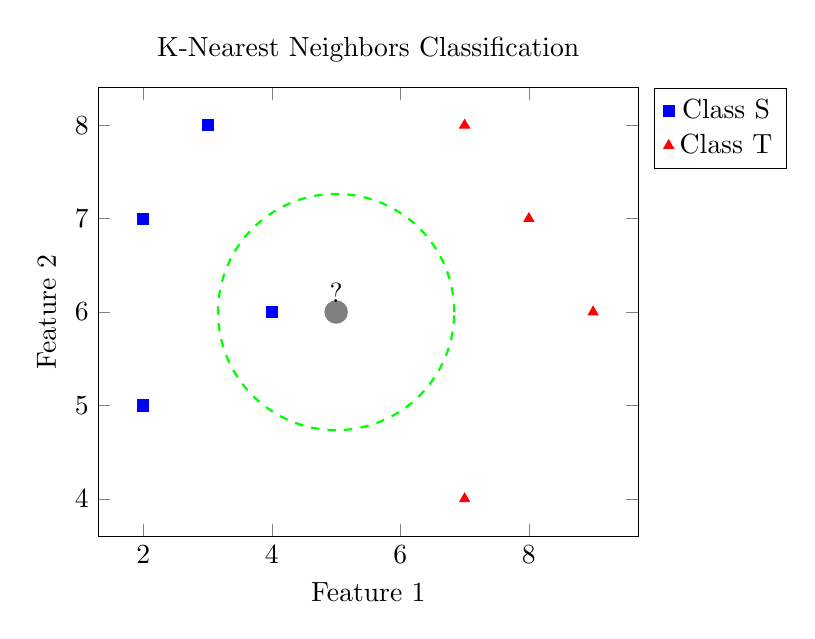
\begin{tikzpicture}
\begin{axis}[
    title={K-Nearest Neighbors Classification},
    xlabel={Feature 1},
    ylabel={Feature 2},
    legend pos=outer north east,
    ]
    % Class S (Squares)
    \addplot[only marks, mark=square*, blue] table {
        x y
        2 7
        3 8
        2 5
        4 6
    };
    \addlegendentry{Class S}
    
    % Class T (Triangles)
    \addplot[only marks, mark=triangle*, red] table {
        x y
        7 8
        8 7
        9 6
        7 4
    };
    \addlegendentry{Class T}
    
    % New point
    \node[circle, fill=gray, inner sep=3pt] at (axis cs:5, 6) (newpoint) {};
    \node[above] at (newpoint) {?};
    
    % k=3 neighbors
    \draw[dashed, green, thick] (axis cs:5, 6) circle [radius=1.5cm];
    \node at (axis cs:8,9) [text=green!50!black] {$k=3$};
\end{axis}
\end{tikzpicture}
\caption{Classifying a new point with KNN (k=3).}
\end{figure}

Here's the entire KNN algorithm:
\begin{enumerate}
    \item \textbf{Calculate Distance:} Measure the distance from our new point (o) to every single other point in the dataset.
    \item \textbf{Find Neighbors:} Find the $k$ closest points. $k$ is a number we choose. Let's say we pick $k=3$. The 3 nearest neighbors are two squares (S) and one triangle (T).
    \item \textbf{Vote!} Have the $k$ neighbors vote on the class. In our $k=3$ example, the vote is 2-to-1 in favor of 'Square'. So, our new point is classified as a blue square. If we had picked $k=5$, the 5 nearest neighbors might be three triangles and two squares, and the point would be classified as a red triangle.
\end{enumerate}
The choice of $k$ is crucial. It's a hyperparameter we have to tune.

\section{From-Scratch Implementation: Let's Get Building}

We're going to build this lazy beast from scratch. The core components are a distance function and a prediction function.

\subsection{1. Distance Metrics: How We Travel}

The concept of "closest" depends on how you measure distance. The two most common ways are \textbf{Euclidean} and \textbf{Manhattan} distance.

\begin{description}
    \item[Euclidean Distance:] "As the crow flies." It's the straight-line distance between two points. You probably remember the formula from school: $\sqrt{(x_2 - x_1)^2 + (y_2 - y_1)^2}$. This is the default for most problems where features are continuous and comparable.
    \item[Manhattan Distance:] "The Taxicab distance." Imagine you're in a city with a perfect grid layout. You can't cut through buildings; you have to travel along the blocks. The Manhattan distance is the sum of the absolute differences along each axis: $|x_2 - x_1| + |y_2 - y_1|$. This is often better for high-dimensional data or when your features are on different, non-comparable scales (e.g., age in years and income in dollars).
\end{description}

\begin{lstlisting}[language=Python]
import numpy as np

def euclidean_distance(point1, point2):
    return np.sqrt(np.sum((point1 - point2)**2))

def manhattan_distance(point1, point2):
    return np.sum(np.abs(point1 - point2))
\end{lstlisting}

\subsection{2. The \texttt{predict()} Function}

This function will orchestrate the whole process.

\begin{lstlisting}[language=Python]
from collections import Counter

def predict_knn(X_train, y_train, new_point, k, distance_metric=euclidean_distance):
    # 1. Calculate distances from the new point to all training points
    distances = [distance_metric(new_point, x) for x in X_train]
    
    # 2. Find the k nearest neighbors
    # We get the indices of the k smallest distances
    k_nearest_indices = np.argsort(distances)[:k]
    
    # Get the labels of those neighbors
    k_nearest_labels = [y_train[i] for i in k_nearest_indices]
    
    # 3. Vote!
    # Counter is a handy way to count the occurrences of each label
    most_common = Counter(k_nearest_labels).most_common(1)
    
    return most_common[0][0]
\end{lstlisting}

And that's it! A fully functional KNN classifier. So simple, so elegant. What could possibly go wrong?

\section{The Curse of Dimensionality: Lost in High-Dimensional Space}

Here's KNN's Achilles' heel. The algorithm relies entirely on the idea of "distance." But what happens to distance when you have a lot of features (dimensions)?

\textbf{Analogy: Finding Your Friend}
\begin{itemize}
    \item \textbf{1 Dimension:} Your friend is somewhere on a 100-meter line. You can probably find them pretty quickly.
    \item \textbf{2 Dimensions:} Your friend is somewhere on a 100m x 100m field. It's harder, but the concept of "nearby" still makes sense.
    \item \textbf{3 Dimensions:} Your friend is in a 100m x 100m x 100m building. Now it's getting really tough.
    \item \textbf{1000 Dimensions:} Your friend is in a 1000-dimensional hypercube. Good luck. You'll never see them again.
\end{itemize}

This is the \textbf{Curse of Dimensionality}. As you add more dimensions, the volume of the space increases exponentially. Your data points, which might have been dense in a few dimensions, become incredibly sparse. Everything becomes far away from everything else. The concept of a "nearest neighbor" becomes meaningless because even your closest neighbor might be astronomically far away.

This isn't just a problem for KNN; it's a fundamental challenge in all of machine learning. It's the reason why simply adding more features to your model often makes it worse, not better. It increases the risk of finding random, meaningless patterns (overfitting) and breaks algorithms that rely on distance. This is the primary motivation for an entire subfield of ML dedicated to \textbf{dimensionality reduction}—techniques that try to squash high-dimensional data down to a lower-dimensional space while preserving the important information.

So while KNN is simple and effective in low dimensions, it gets lost in space as your feature count grows.

\begin{challengebox}
Find the Right K

Let's explore the most important hyperparameter in KNN: $k$.

Grab a standard dataset like the Iris or Breast Cancer dataset from \texttt{sklearn.datasets}.

Split it into a training and testing set.

Using your from-scratch \texttt{predict\_knn} function, write a loop that trains and evaluates the model for different values of $k$ (from 1 to, say, 21, using only odd numbers to avoid ties).

For each $k$, calculate the accuracy on the test set.

Plot the accuracy as a function of $k$.

Analyze the plot:
\begin{itemize}
    \item What happens when $k=1$? Is the accuracy high or low? Why might this be a case of high variance (overfitting)?
    \item What happens when $k$ is very large (e.g., the size of the entire training set)? What does the model predict every time? Why is this a case of high bias (underfitting)?
\end{itemize}
You've just manually plotted your first bias-variance tradeoff curve, one of the most important concepts for debugging any ML model.
\end{challengebox}

\chapter{Naive Bayes: Trust Issues but Make It Statistical}

Alright, let's talk about an algorithm that is simultaneously brilliant, powerful, and built on a foundation of complete and utter delusion.

Meet \textbf{Naive Bayes}.

This algorithm is the workhorse behind many early spam filters. It's a probabilistic classifier that's fast, efficient, and surprisingly effective. And it achieves all this by making one of the most ridiculously bold—and technically wrong—assumptions in all of machine learning. It's like a detective who assumes every suspect in a crime acted completely independently, with no communication or conspiracy whatsoever.

It's a "naive" assumption. But damn, if it doesn't work.

\section{The Core Idea: Bayes' Theorem in Action}

We're going back to Chapter 2 and dusting off our old friend, Bayes' Theorem. As a reminder, it's the formula that lets us update our beliefs in the face of new evidence.
\[ P(A|B) = \frac{P(B|A) \times P(A)}{P(B)} \]
In classification, we want to calculate the probability of a certain class (C) given some observed data (D). For a spam filter, this translates to:
\[ P(\text{Spam}|\text{Email Words}) = \frac{P(\text{Email Words}|\text{Spam}) \times P(\text{Spam})}{P(\text{Email Words})} \]
Let's break this down with a food allergy analogy:
\begin{itemize}
    \item \textbf{P(Spam):} The \textbf{prior probability}. What's the chance that any random email is spam, before we've even read it? Maybe it's 1 in 5 (20\%). This is our starting belief.
    \item \textbf{P(Email Words|Spam):} The \textbf{likelihood}. Given that an email is spam, what's the probability it contains certain words (like "Viagra," "prince," "free")? We can calculate this from our training data.
    \item \textbf{P(Email Words):} The \textbf{evidence}. What's the overall probability of seeing these words in any email, spam or not?
    \item \textbf{P(Spam|Email Words):} The \textbf{posterior probability}. After seeing the words in the email, what is our updated probability that it's spam? This is what we want to calculate.
\end{itemize}
We calculate the posterior probability for both 'Spam' and 'Ham' (not spam). Whichever is higher is our prediction.

\section{The "Naive" Assumption: The Group Project Mentality}

Here's where the magic and the madness come in. Calculating the probability of an entire sentence, like P("free money now"|Spam), is hard because the words aren't independent. The word "money" is more likely to appear if the word "free" is already there.

Naive Bayes says: "LOL, who cares."

It makes the \textbf{class-conditional independence assumption}. It naively assumes that every feature (in this case, every word) is completely independent of every other feature, given the class.

So, instead of a complex calculation, it does this:
\[ P(\text{"free money now"}|\text{Spam}) \approx P(\text{"free"}|\text{Spam}) \times P(\text{"money"}|\text{Spam}) \times P(\text{"now"}|\text{Spam}) \]
This is obviously wrong. In the real world, words have context. "San" is not independent of "Francisco." But this assumption simplifies the math so dramatically that it becomes not just possible, but incredibly fast. It's the ultimate "good enough" engineering tradeoff: sacrifice theoretical purity for practical speed and effectiveness. It's the algorithm equivalent of assuming everyone in a group project will do their part without coordinating—a naive hope, but it simplifies planning.

\section{From-Scratch Spam Filter: Let's Catch Some Scammers}

Let's build a text classifier from the ground up.

\subsection{Step 1: Data Preparation and Training}

The "training" phase for Naive Bayes is just counting.
\begin{enumerate}
    \item Take a dataset of emails already labeled spam or ham.
    \item Calculate the prior probabilities: P(Spam) and P(Ham). This is just (number of spam emails) / (total emails) and (number of ham emails) / (total emails).
    \item Create a vocabulary of all unique words in the dataset.
    \item For each word in the vocabulary, calculate its likelihood for each class. For example:
    \[ P(\text{"Viagra"}|\text{Spam}) = \frac{\text{count of "Viagra" in all spam emails}}{\text{total word count in all spam emails}} \]
    \[ P(\text{"Viagra"}|\text{Ham}) = \frac{\text{count of "Viagra" in all ham emails}}{\text{total word count in all ham emails}} \]
    \item Store all these probabilities in a dictionary or hash map. That's our "trained" model.
\end{enumerate}

\subsection{Step 2: The Problem of Zero Probability \& Laplace Smoothing}

What happens if our new email contains a word the model has never seen before, like "blockchain-crypto-nft-bonanza"? The count for this word would be 0, making its probability 0. When we multiply all the probabilities together, the entire calculation becomes 0, and our model breaks.

To fix this, we use \textbf{Laplace Smoothing} (or add-one smoothing). It's a simple trick: we pretend we've seen every word in our vocabulary one more time than we actually have.

The updated formula becomes:
\[ P(\text{word}|\text{Class}) = \frac{\text{count(word, Class)} + 1}{\text{total words in Class} + \text{size of vocabulary}} \]
This ensures that no word ever has a zero probability. It's like giving every word a tiny head start.

\subsection{Step 3: The \texttt{predict()} function}

Now, to classify a new, unseen email:
\begin{enumerate}
    \item Start with the prior probabilities for 'Spam' and 'Ham'.
    \item For each word in the new email, multiply the running probability by the word's likelihood for that class (e.g., $P(\text{word}|\text{Spam})$).
\end{enumerate}
\textbf{Pro Tip:} Since we're multiplying lots of small probabilities, we can run into floating-point underflow (the numbers get too small for the computer to handle). The standard trick is to use the log of the probabilities instead. Multiplication becomes addition, which is numerically much more stable:
\[ \log(P(\text{Class})) + \sum \log(P(\text{word}_i|\text{Class})) \]
Compare the final log-probability scores for 'Spam' and 'Ham'. The class with the higher score is our prediction.

This approach reveals a powerful engineering principle: sometimes, a model that is technically "wrong" in its assumptions can be more useful in practice than a "correct" model that is too slow or complex to be feasible. Naive Bayes is a triumph of pragmatism over purity, and a testament to the power of a "lazy genius" shortcut.

\begin{challengebox}
Sentiment Analyzer

Your mission is to repurpose our spam filter for a new task: sentiment analysis.

Find a dataset of movie reviews labeled as 'positive' or 'negative'. The IMDB dataset from is a classic choice.

Adapt your from-scratch Naive Bayes code. Instead of 'spam' and 'ham', your classes are now 'positive' and 'negative'.

Train your model on the review data.

After training, find the top 10 words with the highest likelihood for the 'positive' class and the top 10 for the 'negative' class. Do they make sense?

Write a function that takes a new review (a string) and predicts whether its sentiment is positive or negative. Test it out!
\end{challengebox}

\chapter{Clustering: Group Therapy for Data}

So far, we've lived in the cozy, well-lit world of supervised learning. We've always had an answer key. Our data was neatly labeled, and our job was to teach a model to predict those labels.

Now, we're turning off the lights.

Welcome to unsupervised learning. Here, we have no labels. No right answers. We just have a chaotic mess of data points, and our job is to find the natural structure within them. We're not predicting; we're discovering.

The most fundamental task in unsupervised learning is \textbf{clustering}: finding the natural "cliques" or "groups" in your data. And the king of clustering algorithms is \textbf{K-Means}.

\section{The Goal: Finding the Cliques}

Imagine you're a high school principal looking at a map of where all your students hang out during lunch. You don't have pre-defined labels like "jocks" or "nerds." You just see a scatter plot of students. Your goal is to identify the main social groups. You'd probably circle the dense clumps of students, right?

That's exactly what K-Means does. It's an algorithm designed to partition your data into a pre-defined number ($k$) of clusters.

\section{The K-Means Algorithm: A Ghosting Story}

The K-Means algorithm is a beautiful, iterative dance. It's like forcing your data points into group therapy sessions until they find where they truly belong. Here's how it works, told as a story of ghosting centroids:
\begin{description}
    \item[Step 1: Initialize (The Awkward Mixer).] You decide you want to find $k$ groups (let's say $k=3$). To start, you pluck $k$ random data points from your dataset and call them \textbf{centroids}. These are the initial, randomly chosen "group leaders." They stand awkwardly in the middle of the room.
    \item[Step 2: Assign (Find Your Clique).] Go through every single data point. For each point, calculate its distance to all three centroids. Assign the data point to the group of the centroid it's closest to. Now you have three distinct clusters of points, each huddled around their initial leader.
    \item[Step 3: Update (The Centroid Ghosts).] Now, the centroids look at the new group of friends they've attracted. They say, "I should be in the middle of my new friend group." So, each centroid calculates the \textbf{mean} (the average position) of all the data points in its cluster and moves to that new position. It ghosts its old location and reappears in the center of its clique.
    \item[Step 4: Repeat.] Now that the centroids have moved, some data points might be closer to a different centroid. So, you repeat Step 2 (re-assign all points to their new closest centroid). Then you repeat Step 3 (update the centroids to their new mean position).
\end{description}
You keep repeating this Assign-Update loop until the centroids stop moving. When a full loop happens and no data points change their cluster assignment, the algorithm has \textbf{converged}. The groups are stable. The therapy session is over.

\section{From-Scratch K-Means: Let's Make Some Clusters}

You know the drill. Let's build it. The core of K-Means is a loop that contains our two main steps.

\begin{lstlisting}[language=Python]
import numpy as np
import matplotlib.pyplot as plt

# We'll reuse our distance function from Chapter 7
def euclidean_distance(point1, point2):
    return np.sqrt(np.sum((point1 - point2)**2))

def kmeans(X, k, max_iters=100):
    # 1. Initialize centroids randomly from the data
    num_samples, num_features = X.shape
    random_indices = np.random.choice(num_samples, k, replace=False)
    centroids = X[random_indices, :]

    for _ in range(max_iters):
        # 2. Assign each data point to the closest centroid
        clusters = [[] for _ in range(k)]
        for idx, sample in enumerate(X):
            distances = [euclidean_distance(sample, point) for point in centroids]
            closest_centroid_idx = np.argmin(distances)
            clusters[closest_centroid_idx].append(idx)

        # Store old centroids to check for convergence
        old_centroids = centroids.copy()

        # 3. Update centroids to be the mean of their assigned points
        for i in range(k):
            if clusters[i]: # Avoid empty clusters
                cluster_points = X[clusters[i]]
                centroids[i] = np.mean(cluster_points, axis=0)

        # 4. Check for convergence
        if np.all(centroids == old_centroids):
            break
            
    # Return the final cluster assignments and centroids
    labels = np.empty(num_samples)
    for i, cluster in enumerate(clusters):
        labels[cluster] = i
        
    return labels, centroids
\end{lstlisting}

Visualizing this process is incredibly satisfying. You can plot the data points and watch the centroids dance around with each iteration until they settle into the heart of their clusters.

\section{The Elbow Method: Finding the Sweet Spot (Unlike Your Ex)}

There's a huge question we've been ignoring: how do you pick $k$? Why 3 clusters and not 2, or 10?

This is a common problem in unsupervised learning. Since there's no "right" answer, we have to use a heuristic. The most popular one is the \textbf{Elbow Method}.

\textbf{Analogy: The Law of Diminishing Returns}

Imagine you're cleaning a messy room.
\begin{itemize}
    \item Adding one trash can ($k=1$) helps a lot. Huge improvement.
    \item Adding a second trash can ($k=2$) for recycling also helps a lot.
    \item Adding a third ($k=3$) might still be useful.
    \item Adding a tenth ($k=10$)? At this point, you're just adding more trash cans for the sake of it. The improvement is tiny.
\end{itemize}
The Elbow Method does the same for clusters. We calculate a score called the \textbf{Within-Cluster Sum of Squares (WCSS)}. This is just the sum of the squared distances between each point and its centroid. It's a measure of how tight and compact the clusters are. A lower WCSS is better.

We run K-Means for a range of $k$ values (e.g., $k=1$ to $k=10$) and plot the WCSS for each. The graph will look like an arm bending downwards.

\begin{figure}[h!]
\centering
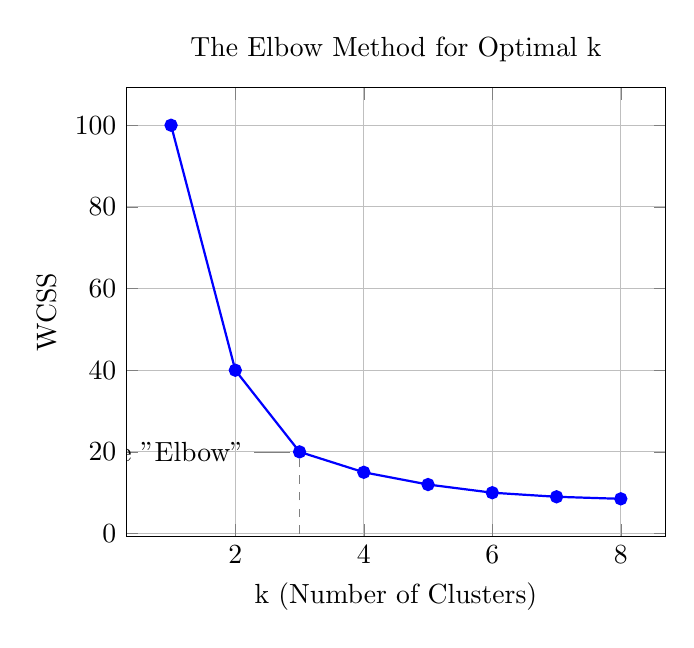
\begin{tikzpicture}
\begin{axis}[
    title={The Elbow Method for Optimal k},
    xlabel={k (Number of Clusters)},
    ylabel={WCSS},
    grid=major,
    ]
    \addplot[mark=*, blue, thick] coordinates {
        (1, 100)
        (2, 40)
        (3, 20)
        (4, 15)
        (5, 12)
        (6, 10)
        (7, 9)
        (8, 8.5)
    };
    \node[pin=180:{The "Elbow"}] at (axis cs:3, 20) {};
    \draw[gray, dashed] (axis cs:3,0) -- (axis cs:3,20);
\end{axis}
\end{tikzpicture}
\caption{Finding the optimal k using the Elbow Method (Fixed).}
\end{figure}

The "elbow" of the arm is the point where the WCSS stops decreasing so rapidly. It's the point of diminishing returns, where adding another cluster doesn't give you much bang for your buck. This is our best guess for the optimal value of $k$.

It's important to recognize that the random initialization of centroids can be a significant weakness. A bad start can cause the algorithm to converge to a local minimum—a solution that is good, but not the best possible one. This is the same "stuck in a shallow valley" problem we saw with gradient descent. To combat this, standard implementations of K-Means (like the one in \texttt{sklearn}) run the entire algorithm multiple times with different random starting points (\texttt{n\_init}) and then pick the best final result.

\begin{challengebox}
Image Compression with K-Means

Let's use clustering for something cool and visual: color quantization, a form of image compression.

Load an image using a library like Pillow or OpenCV.

The image is a 3D array (height, width, RGB channels). Reshape it into a 2D array where each row is a pixel and the columns are its Red, Green, and Blue values. This is your $X$ data.

Use your from-scratch K-Means algorithm to find, say, $k=16$ clusters in this pixel data. The final centroids will be the 16 most representative colors in the image.

Create a new image by replacing each original pixel's color with the color of the centroid it was assigned to.

Display the original and the new, compressed image side-by-side. You've just reduced the number of colors in the image to 16, effectively compressing it!
\end{challengebox}

\chapter{Intro to Neural Networks: Baby’s First Brain}

Alright, we've built models that can draw lines, ask questions, and find cliques. We've been building with Lego bricks. Now it's time to build the Death Star.

Welcome to \textbf{Neural Networks}.

These are the models that power everything from self-driving cars to generating art to translating languages. They look terrifyingly complex from the outside, like a diagram of the entire internet. But here's the secret: a neural network is just layers upon layers of the simple things we've already learned.

Let's demystify the beast and build our own tiny brain.

\section{The Neuron (Perceptron): Not Actually Brain Surgery}

The basic building block of a neural network is a \textbf{neuron}, also known as a \textbf{perceptron}. And a single neuron is going to look incredibly familiar. It's basically just a logistic regression unit.

Here's what a neuron does:
\begin{enumerate}
    \item It takes one or more inputs ($x_1, x_2, ...$).
    \item It calculates a weighted sum of those inputs and adds a bias: $z = (w_1x_1 + w_2x_2 + ...) + b$. (Sound familiar? It's the linear regression equation.)
    \item It passes this result, $z$, through an \textbf{activation function}. (Sound familiar? It's what we did in logistic regression.)
\end{enumerate}
That's it. A single neuron is just a simple linear model followed by a non-linear activation.

\section{Activation Functions: The Neuron's Mood Ring}

The activation function is what gives the network its power. It decides whether the neuron "fires" and what signal it sends to the next layer. Without it, a neural network would just be a massive, useless linear regression model. Here are the three A-listers you need to know:
\begin{description}
    \item[Sigmoid:] The OG. We met it in Chapter 5. It squishes any number into a (0, 1) range.
    \begin{itemize}
        \item \textbf{Use Case:} Great for the final output layer in a binary classification problem, because it gives you a probability.
        \item \textbf{Problem:} Suffers from the "vanishing gradient" problem. The curve gets very flat at the ends, meaning the derivative is close to zero. This can cause learning to grind to a halt in deep networks.
    \end{itemize}
    \item[Tanh (Hyperbolic Tangent):] Sigmoid's cooler, zero-centered sibling. It squishes numbers into a (-1, 1) range.
    \begin{itemize}
        \item \textbf{Use Case:} Often performs better than sigmoid in hidden layers because its output is centered around zero, which can help with optimization.
        \item \textbf{Problem:} Still suffers from the vanishing gradient problem at the ends.
    \end{itemize}
    \item[ReLU (Rectified Linear Unit):] The undisputed king of modern deep learning. Its function is hilariously simple:
    \[ f(x) = \max(0, x) \]
    If the input is positive, it passes it through unchanged. If it's negative, it just outputs zero.
    \begin{itemize}
        \item \textbf{Use Case:} The default, go-to activation function for almost all hidden layers.
        \item \textbf{Advantages:} It's incredibly fast to compute (no fancy exponents). More importantly, for positive values, the slope is a constant 1. This means the gradient doesn't vanish, allowing models to learn much faster and deeper.
    \end{itemize}
\end{description}

\section{The Network: Stacking Layers of Neurons}

A single neuron is dumb. But what happens when we connect them? We get a network.

\begin{figure}[h!]
\centering
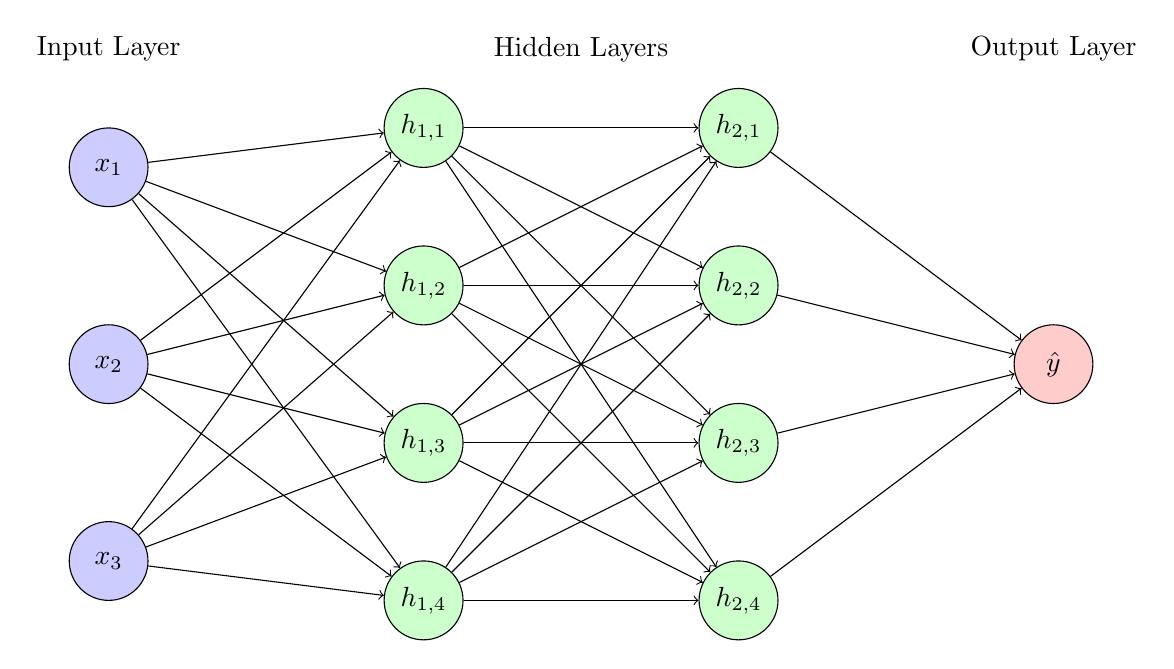
\begin{tikzpicture}[
    neuron/.style={circle, draw, minimum size=1cm},
    input/.style={neuron, fill=blue!20},
    hidden/.style={neuron, fill=green!20},
    output/.style={neuron, fill=red!20},
]
    % Input Layer
    \foreach \i in {1,...,3}
        \node[input] (I-\i) at (0, -2.5*\i) {$x_\i$};
    
    % Hidden Layer 1
    \foreach \i in {1,...,4}
        \node[hidden] (H1-\i) at (4, -2*\i) {$h_{1,\i}$};
        
    % Hidden Layer 2
    \foreach \i in {1,...,4}
        \node[hidden] (H2-\i) at (8, -2*\i) {$h_{2,\i}$};

    % Output Layer
    \node[output] (O-1) at (12, -5) {$\hat{y}$};
    
    % Connections
    \foreach \i in {1,...,3}
        \foreach \j in {1,...,4}
            \draw[->] (I-\i) -- (H1-\j);
            
    \foreach \i in {1,...,4}
        \foreach \j in {1,...,4}
            \draw[->] (H1-\i) -- (H2-\j);

    \foreach \i in {1,...,4}
        \draw[->] (H2-\i) -- (O-1);
        
    % Labels
    \node at (0, -1) {Input Layer};
    \node at (6, -1) {Hidden Layers};
    \node at (12, -1) {Output Layer};
\end{tikzpicture}
\caption{A simple feedforward neural network architecture.}
\end{figure}

A neural network is just neurons organized in layers:
\begin{itemize}
    \item An \textbf{Input Layer:} Receives the raw data (e.g., the pixel values of an image, the features of a house).
    \item One or more \textbf{Hidden Layers:} These are the intermediate layers where the real "thinking" happens. The output of one layer becomes the input for the next.
    \item An \textbf{Output Layer:} Produces the final prediction (e.g., a single neuron with a sigmoid for binary classification, or multiple neurons for multi-class problems).
\end{itemize}
This layering is what allows the network to learn hierarchical patterns. The first layer might learn to recognize simple edges. The next layer might combine those edges to recognize shapes like eyes and noses. The final layer might combine those shapes to recognize a face.

\section{Forward \& Backpropagation: The Matrix Moment}

How does a network actually learn? It's a two-step dance called \textbf{Forward} and \textbf{Backward Propagation}.

\subsection{1. Forward Propagation (The Easy Part)}

This is just the process of making a prediction. You feed your input data into the first layer. The neurons do their thing (weighted sum + activation) and pass their outputs to the next layer. This continues layer by layer until you get a final output from the output layer. It's one giant, nested function call.

\subsection{2. Backpropagation (The "Magic")}

This is where the learning happens. After the forward pass, you have a prediction. You compare it to the true label using a loss function (like MSE or Binary Cross-Entropy) to get a single error number.

Now, we need to figure out which of the thousands (or millions) of weights in the network was responsible for the error. \textbf{Backpropagation} is the algorithm that does this.

It's just the \textbf{chain rule} from calculus, applied cleverly and efficiently.
\begin{enumerate}
    \item It starts at the end, with the loss. It calculates the gradient of the loss with respect to the weights in the last layer.
    \item Then, it moves one layer back. It uses the gradients it just calculated to figure out the gradients for the weights in the second-to-last layer.
    \item It continues this process, propagating the error signal backwards through the network, layer by layer, until it has calculated the gradient (the "blame") for every single weight and bias.
\end{enumerate}
Once you have all the gradients, you just use our old friend Gradient Descent to update every weight and bias in the network, taking a tiny step in the direction that will lower the loss.
\[ \text{weight} = \text{weight} - \text{learning\_rate} \times \text{gradient} \]
That's the entire training loop: Forward Pass $\rightarrow$ Calculate Loss $\rightarrow$ Backward Pass (Backpropagation) $\rightarrow$ Update Weights. Repeat 10,000 times.

\section{From-Scratch XOR Solver: The "Aha!" Moment}

Remember the XOR problem from Chapter 5 that our linear logistic regression model couldn't solve? A single straight line can't separate the XOR data.

But a neural network can. By using a hidden layer, the network can learn to draw more complex, non-linear decision boundaries. The first layer might learn two different lines, and the output layer can learn to combine the results of those lines in a non-linear way (like an AND or OR operation) to create a boundary that perfectly solves XOR.

This is the superpower of neural networks. They are \textbf{universal function approximators}, which is a fancy way of saying that a network with at least one hidden layer and enough neurons can, in theory, learn to approximate any continuous function. This is why they are so powerful and versatile.

Let's prove it. We'll build a tiny neural network from scratch to finally conquer the XOR problem.

\begin{lstlisting}[language=Python]
# A tiny NN to solve XOR
# Input layer: 2 neurons
# Hidden layer: 2 neurons (with ReLU activation)
# Output layer: 1 neuron (with Sigmoid activation)

# We'll need to define our layers, weights, biases...
# ...and then implement the full training loop:
# for epoch in range(epochs):
#     1. Forward pass
#     2. Calculate loss
#     3. Backpropagation to get gradients
#     4. Update weights and biases with gradient descent
\end{lstlisting}

When you run this code, you'll see the loss drop and the model learn to correctly classify all four XOR points. It's the moment you realize that by stacking simple components, you can create something with truly powerful capabilities.

\begin{challengebox}
The Activation Function Gauntlet

Let's see the impact of our activation functions firsthand.

Take the from-scratch XOR solver we just built.

Train it three times, each time using a different activation function for the hidden layer:
\begin{itemize}
    \item Sigmoid
    \item Tanh
    \item ReLU
\end{itemize}
For each run, keep track of the loss at every epoch.

Plot the three loss curves on the same graph.

Analyze the results: Which activation function allowed the network to learn the fastest (i.e., its loss dropped most quickly)? Which one performed the best overall? You'll see with your own eyes why ReLU is the default choice for hidden layers in almost every modern neural network.
\end{challengebox}

\part{LET’S BUILD THINGS (Projects \& Fun Stuff)}

\chapter{ML Playground: Code Like You Mean It}

Alright, enough theory. You've built the engines, you understand the mechanics, you've stared into the mathematical abyss and didn't blink. Theory's over. Time to build cool shit.

In this chapter, we're taking our beautiful, hand-crafted, from-scratch models out for a spin. We're going to point them at real-world (and slightly ridiculous) problems and make them do something. This is where the rubber meets the road. Or, more accurately, where the \texttt{predict()} function meets the CSV file.

We'll walk through a few mini-projects, covering the essential pipeline: loading data, a bit of cleaning, training our DIY models, and trying to make sense of the results.

\section{Project 1: Predicting Spotify Song Popularity}

\begin{description}
    \item[The Goal:] Can we predict how popular a song will be?
    \item[The Dataset:] We'll use a Spotify dataset from Kaggle, which has audio features for thousands of songs. It includes things like 'danceability', 'energy', 'loudness', and a 'popularity' score from 0-100.
    \item[Our Weapon of Choice:] The output, 'popularity', is a continuous number. This is a classic regression problem. We'll use our DIY Linear Regression model from Chapter 4.
    \item[The Workflow:]
    \begin{enumerate}
        \item \textbf{Load Data:} We'll use the pandas library to load the \texttt{spotify\_songs.csv} file into a DataFrame.
        \item \textbf{Feature Selection:} We can't throw everything at our simple model. Let's pick a few features that seem intuitive, like \texttt{danceability} and \texttt{energy}. Our X will be these two columns, and our y will be the \texttt{popularity} column.
        \item \textbf{Train the Model:} We'll feed our X and y data into the training loop for our from-scratch linear regression model. It will chug away and find the best weights (coefficients) for \texttt{danceability} and \texttt{energy}, plus a bias term.
        \item \textbf{Interpret the Results:} Our trained model will give us an equation like:
        \[ \text{popularity} = (w_1 \times \text{danceability}) + (w_2 \times \text{energy}) + b \]
        We can look at the weights! If $w_1$ is large and positive, it means our model learned that higher danceability strongly correlates with higher popularity.
    \end{enumerate}
\end{description}

\section{Project 2: Is This Tweet Trash or Fire? (Sentiment Analysis)}

\begin{description}
    \item[The Goal:] Classify a tweet's sentiment as either 'positive' or 'negative'.
    \item[The Dataset:] We'll grab a simple Twitter sentiment analysis dataset, which contains tweets labeled with their sentiment.
    \item[Our Weapon of Choice:] We're classifying text. This is the home turf of our DIY Naive Bayes classifier from Chapter 8.
    \item[The Workflow:]
    \begin{enumerate}
        \item \textbf{Load Data:} Load the CSV of tweets and labels.
        \item \textbf{Text Preprocessing:} Real-world text is messy. We'll need to do some basic cleaning:
        \begin{itemize}
            \item Convert all text to lowercase.
            \item Remove punctuation and URLs.
            \item Split the text into individual words (tokenization).
        \end{itemize}
        \item \textbf{Train the Model:} We'll feed our cleaned-up tweets and their labels ('positive'/'negative') into our Naive Bayes trainer. It will count word frequencies for each class and calculate the prior probabilities and likelihoods, just like we did for the spam filter.
        \item \textbf{Test It Out:} We'll write a new, unseen tweet like "this movie was absolutely incredible" and see if our model correctly predicts 'positive'. Then we'll try "I would rather watch paint dry" and see if it predicts 'negative'.
    \end{enumerate}
\end{description}

\section{Project 3: Recommending Snacks Based on Mood (No, Seriously)}

\begin{description}
    \item[The Goal:] Build a highly scientific model to recommend the perfect snack for your current mood.
    \item[The Dataset:] We're going to create this one ourselves. It's a testament to the fact that you can do machine learning on anything.
    \begin{table}[h!]
    \centering
    \begin{tabular}{llll}
    \hline
    \textbf{Mood} & \textbf{Weather} & \textbf{Time of Day} & \textbf{Snack} \\
    \hline
    Stressed & Rainy & Evening & Chocolate \\
    Bored & Sunny & Afternoon & Chips \\
    Happy & Sunny & Morning & Fruit \\
    Stressed & Sunny & Afternoon & Chocolate \\
    Tired & Rainy & Evening & Ice Cream \\
    Bored & Cloudy & Evening & Popcorn \\
    \hline
    \end{tabular}
    \end{table}
    \item[Our Weapon of Choice:] This is a simple, multi-class classification problem with categorical features. It's a perfect, low-dimensional use case for our DIY K-Nearest Neighbors model from Chapter 7.
    \item[The Workflow:]
    \begin{enumerate}
        \item \textbf{Data Prep:} We need to convert our categorical features into numbers. We can do a simple mapping: stressed=0, bored=1, happy=2, etc.
        \item \textbf{"Train" the Model:} For KNN, "training" just means storing this tiny dataset in memory.
        \item \textbf{Make a Prediction:} Let's say our new situation is \texttt{mood='stressed'}, \texttt{weather='cloudy'}, \texttt{time='evening'}. We convert this to numbers, find the $k$ nearest neighbors in our dataset (maybe $k=1$ is best for this tiny dataset), and see what they were eating. The model will likely find that the closest neighbor is (Stressed, Rainy, Evening) and recommend Chocolate. Science!
    \end{enumerate}
\end{description}

\section{Building Your First ML Pipeline}

As we do these projects, we'll notice a repeating pattern. We'll formalize it by creating a simple Python class that represents our first ML pipeline:

\begin{lstlisting}[language=Python]
class SimpleMLPipeline:
    def __init__(self, model):
        self.model = model

    def load_data(self, filepath):
        #... pandas logic to load CSV
        pass

    def clean_data(self, data):
        #... logic to handle missing values, etc.
        pass

    def train(self, X, y):
        self.model.fit(X, y) # Assuming our models have a .fit() method

    def evaluate(self, X_test, y_test):
        #... logic to calculate accuracy/loss
        pass
\end{lstlisting}

This exercise demonstrates a crucial real-world concept: the choice of algorithm is driven by the problem you're trying to solve and the kind of data you have. There is no single "best" algorithm. A linear model is great for continuous outputs, Naive Bayes excels at text, and KNN can be surprisingly effective for simple, low-dimensional classification. Moving from knowing how an algorithm works to knowing when to use it is the leap from being a student to being a practitioner.

\begin{challengebox}
Choose Your Own Adventure

Your turn to be the data scientist.
\begin{enumerate}
    \item Go to Kaggle or another dataset repository and find a dataset that looks fun to you. Some ideas: "Wine Quality Prediction," "Video Game Sales," "IMDB TV Show Reviews."
    \item \textbf{Define the problem:} What are you trying to predict? Is it a regression or classification task?
    \item \textbf{Choose your weapon:} Pick one of our from-scratch models (Linear Regression, Logistic Regression, KNN, Naive Bayes, or Decision Tree) that you think is best suited for the job.
    \item Write a simple Python script to load the data, train your chosen model, and make a few predictions.
    \item \textbf{Justify your choice:} In a code comment, write a few sentences explaining why you chose that specific model for that specific problem.
\end{enumerate}
\end{challengebox}

\chapter{When Your Model Screws Up (And Why It’s Your Fault)}

So, you've built a model. You fed it data, you watched the loss curve go down, and you got a prediction. You might have even calculated its accuracy and seen a glorious 99\% printed to your console.

Time to deploy to production and become a billionaire, right?

Wrong.

Welcome to the most important chapter in this book. This is where we talk about debugging. Because your model might have 99\% accuracy and still be complete and utter garbage. And when your model screws up, there's one person to blame: you.

\section{Overfitting vs. Underfitting: The Student Analogy}

The most common failure modes for a model are \textbf{overfitting} and \textbf{underfitting}. They represent two sides of the same coin: the model's ability to generalize from the training data to new, unseen data.

\begin{description}
    \item[Underfitting (High Bias): The Lazy Student]
    \begin{itemize}
        \item \textbf{The Symptom:} The model performs poorly on the training data \emph{and} the test data.
        \item \textbf{The Analogy:} This is the student who didn't study at all. They don't know the material, so they fail the practice questions and they fail the final exam.
        \item \textbf{The Cause:} The model is too simple to capture the underlying patterns in the data. Using a linear model to describe a complex, curvy relationship is a classic example of underfitting.
        \item \textbf{The Fix:} Use a more complex model! If a straight line isn't working, try a polynomial, or a deep decision tree, or a neural network.
    \end{itemize}
    \item[Overfitting (High Variance): The Memorizing Nerd]
    \begin{itemize}
        \item \textbf{The Symptom:} The model performs perfectly on the training data but falls apart on the test data.
        \item \textbf{The Analogy:} This is the student who didn't learn the concepts, they just memorized the exact answers to the 50 questions in the study guide. They get 100\% on the study guide, but when the final exam asks slightly different questions, they are completely lost.
        \item \textbf{The Cause:} The model is too complex. It has learned not only the signal in the training data, but also the \emph{noise}. It has fit itself to the random quirks of the specific data points it saw, instead of the general trend. A decision tree with no \texttt{max\_depth} is a classic overfitter.
        \item \textbf{The Fix:} Simplify the model! Use regularization, prune your decision tree, or get more training data.
    \end{itemize}
\end{description}

This meme explains overfitting better than any textbook could:

\begin{figure}[h!]
    \centering
    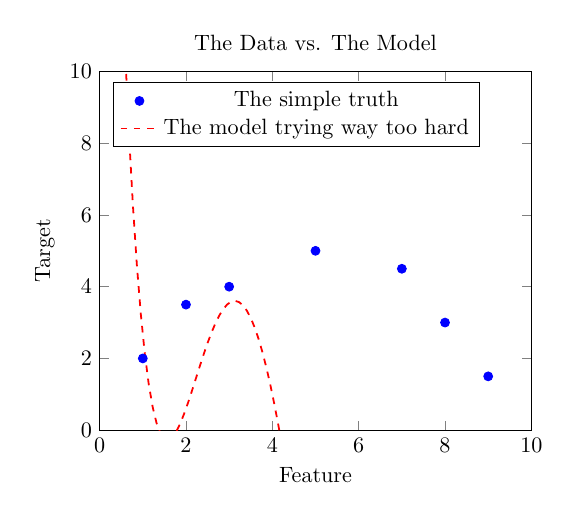
\begin{tikzpicture}[scale=0.8, transform shape]
        \begin{axis}[
            title={The Data vs. The Model},
            xmin=0, xmax=10, ymin=0, ymax=10,
            xlabel={Feature}, ylabel={Target},
            legend pos=north west
        ]
            % The actual data points
            \addplot[only marks, mark=*, blue] coordinates {
                (1, 2) (2, 3.5) (3, 4) (5, 5) (7, 4.5) (8, 3) (9, 1.5)
            };
            \addlegendentry{The simple truth}

            % The overfit model
            \addplot[red, thick, samples=100, domain=0.5:9.5, dashed] 
                plot (\x, {
                -0.05*\x^5 + 1.2*\x^4 - 10.5*\x^3 + 40*\x^2 - 65*\x + 37
                });
            \addlegendentry{The model trying way too hard}
        \end{axis}
    \end{tikzpicture}
    \caption{A new, improved overfitting meme, made with 100\% LaTeX.}
\end{figure}

The model fits the training data (the blue dots) perfectly. But it won't work for any other data point because it has learned the noise, not the simple underlying curve. It has failed to generalize.

\section{The Bias-Variance Tradeoff: The Goldilocks Problem}

These two problems are fundamentally linked. This is the \textbf{Bias-Variance Tradeoff}, the central tension in supervised learning.
\begin{itemize}
    \item \textbf{Bias} is the error from a model being too simple (underfitting).
    \item \textbf{Variance} is the error from a model being too sensitive to the training data (overfitting).
\end{itemize}
You can't have your cake and eat it too.
\begin{itemize}
    \item If you decrease bias (by making your model more complex), you almost always increase variance.
    \item If you decrease variance (by simplifying your model), you almost always increase bias.
\end{itemize}
The goal is not to eliminate one or the other, but to find the "Goldilocks" spot in the middle—a model that is complex enough to capture the true signal, but not so complex that it starts memorizing the noise.

\section{Cross-Validation: Stop Lying to Yourself}

How do you find this sweet spot? Your simple train-test split is a good start, but what if you just got lucky (or unlucky) with your split?

\textbf{K-Fold Cross-Validation} is the professional's tool for getting a more robust and honest evaluation of model performance.

Here's how it works ($k=5$ is a common choice):
\begin{enumerate}
    \item Shuffle your dataset randomly.
    \item Split it into $k$ equal-sized folds (e.g., 5 folds of 20\% each).
    \item Now, you run 5 experiments:
    \begin{itemize}
        \item \textbf{Run 1:} Train on Folds 1-4, test on Fold 5.
        \item \textbf{Run 2:} Train on Folds 1,2,3,5, test on Fold 4.
        \item \textbf{Run 3:} Train on Folds 1,2,4,5, test on Fold 3.
        \item ...and so on.
    \end{itemize}
\end{enumerate}
You end up with 5 different performance scores. The average of these scores is your cross-validated performance.

This is like giving your student 5 different versions of the final exam and averaging their scores. It gives you a much more reliable estimate of how your model will perform on data it has never seen.

\section{Metrics That Actually Matter: Accuracy is for Amateurs}

Okay, here's the biggest trap for beginners. You build a model, and you see: \texttt{Accuracy: 99.0\%}. You think you're a genius.

But what if you're building a model to detect a rare disease that only affects 1\% of the population? A lazy model that just predicts "No Disease" for every single person will be 99\% accurate. And it will be 100\% useless. It will miss every single person who actually has the disease.

This is why accuracy can be a terrible metric, especially for imbalanced datasets. We need smarter metrics. Enter \textbf{Precision} and \textbf{Recall}.

\textbf{Analogy: The Fishing Net}

Imagine your model is a fishing net. The fish are the positive cases you want to find (e.g., "spam," "disease"). The rocks and seaweed are the negative cases.
\begin{description}
    \item[Precision:] "Of all the stuff in your net, how much is actually fish?"
    \[ \text{Precision} = \frac{\text{True Positives}}{\text{True Positives} + \text{False Positives}} \]
    High precision means your model is very trustworthy when it says something is positive.
    \begin{itemize}
        \item \textbf{When it matters:} Spam filtering. A false positive (a real email going to spam) is much worse than a false negative (a spam email getting through). You want the stuff in the "spam" net to be almost exclusively spam.
    \end{itemize}
    \item[Recall (or Sensitivity):] "Of all the fish in the lake, how many did you catch?"
    \[ \text{Recall} = \frac{\text{True Positives}}{\text{True Positives} + \text{False Negatives}} \]
    High recall means your model is very good at finding all the positive cases.
    \begin{itemize}
        \item \textbf{When it matters:} Medical diagnosis. A false negative (missing a real disease) is catastrophic. You'd rather have a few false positives (telling a healthy person to get more tests) than miss a single case. You want to catch all the fish.
    \end{itemize}
    \item[F1-Score: The Balanced Scorecard]
    \[ \text{F1-Score} = 2 \times \frac{\text{Precision} \times \text{Recall}}{\text{Precision} + \text{Recall}} \]
    The F1-score is the harmonic mean of precision and recall. It's a single number that gives you a balanced measure of both. If either precision or recall is very low, the F1-score will also be low. It's the best default metric for many problems.
\end{description}

Here's your go-to guide:
\begin{table}[h!]
\centering
\begin{tabular}{|p{2.5cm}|p{4.5cm}|p{3cm}|p{3.5cm}|}
\hline
\textbf{Metric} & \textbf{Question it Answers} & \textbf{When to Use It} & \textbf{Real-World Example} \\
\hline
\textbf{Accuracy} & Overall, what fraction of predictions were correct? & Only for balanced datasets where false positives and false negatives have similar costs. & Classifying images of cats vs. dogs (balanced classes). \\
\hline
\textbf{Precision} & When my model predicts YES, how often is it correct? & When the cost of a False Positive is high. & Spam detection, high-stakes investment predictions. \\
\hline
\textbf{Recall} & Of all the actual YES cases, how many did my model find? & When the cost of a False Negative is high. & Medical diagnosis, fraud detection. \\
\hline
\textbf{F1-Score} & How can I get a balanced measure of both Precision and Recall? & When you need a balance between Precision and Recall, or for imbalanced datasets. & Most real-world classification problems. \\
\hline
\end{tabular}
\caption{Choosing the right evaluation metric.}
\end{table}

Stop using accuracy as your only metric. Start thinking about the cost of your model's mistakes. That's how you go from building toys to building tools.

\begin{challengebox}
The Doctor and the Spammer

You are evaluating two different machine learning models for two different jobs.
\begin{itemize}
    \item \textbf{Model A:} 99\% Precision, 40\% Recall.
    \item \textbf{Model B:} 65\% Precision, 98\% Recall.
\end{itemize}
\begin{description}
    \item[Job 1: Cancer Detection System.] You need to build a model that screens patient scans for signs of cancer. Which model do you choose, A or B? Justify your answer in terms of false positives and false negatives.
    \item[Job 2: Email Spam Filter.] You need to build a model that automatically moves spam emails to a junk folder. Which model do you choose, A or B? Justify your answer in terms of false positives and false negatives.
\end{description}
There is a right and a wrong answer for each. Choose wisely.
\end{challengebox}

\chapter{From Scratch to Sklearn: Using Libraries with Dignity}

You've done the hard work. You've implemented gradient descent by hand. You've built a recursive tree-splitter. You've coded up the beautiful, chaotic dance of K-Means centroids. You have stared into the void of backpropagation, and the void stared back.

You have earned the shortcut.

In this chapter, we're going to take our messy, beautiful, educational from-scratch code and refactor it into a few elegant lines of \textbf{scikit-learn}. This isn't cheating. This is graduating.

\section{The "Why": Don't Reinvent the Wheel (Unless You're Learning How Wheels Work)}

Let's be crystal clear. We built these algorithms from scratch for one reason: to understand what the hell is going on under the hood. You now know what a \texttt{learning\_rate} actually does. You know what \texttt{n\_neighbors} in a KNN model represents. You know that a \texttt{DecisionTreeClassifier} is just a machine for finding the best if/else statements.

In the real world, you will almost never implement these algorithms from scratch for a production system. Why? Because libraries like scikit-learn are:
\begin{itemize}
    \item \textbf{Optimized:} Written in low-level languages like C and Cython for maximum speed. Your pure Python loops are charming, but slow.
    \item \textbf{Battle-Tested:} Used and scrutinized by millions of developers. They've found and fixed bugs you haven't even dreamed of.
    \item \textbf{Feature-Rich:} They include advanced solvers, clever initialization tricks (like k-means++), and tons of utility functions that would take you months to build.
\end{itemize}
You built the go-kart from spare parts to learn how an engine works. Now it's time to drive the Formula 1 car.

\section{Refactoring Our Greatest Hits}

Let's see how the pros do it. We're going to take our models from Part 2 and show their sklearn equivalent. The difference will be... striking.

\subsection{1. Linear Regression (Chapter 4)}

\textbf{Our Scratch Code:} \textasciitilde50 lines of Python for \texttt{predict}, \texttt{loss}, \texttt{update}, and a training loop.

\textbf{The Sklearn Way:}
\begin{lstlisting}[language=Python]
from sklearn.linear_model import LinearRegression
import numpy as np

# Same data as before
X = np.array([[2], [3], [5], [6], [8]]) # Sklearn expects a 2D array for X
y_true = np.array([65, 70, 75, 85, 90])

# 1. Instantiate the model
model = LinearRegression()

# 2. Train the model (this does the whole gradient descent thing for you)
model.fit(X, y_true)

# 3. Get the results
print(f"Sklearn m: {model.coef_[0]:.2f}")
print(f"Sklearn b: {model.intercept_:.2f}")

# 4. Make a prediction
print(f"Prediction for 7 hours of study: {model.predict([[7]]):.2f}")
\end{lstlisting}
Three lines. That's it. Our entire chapter's work, condensed.

\subsection{2. K-Nearest Neighbors (Chapter 7)}

\textbf{Our Scratch Code:} \textasciitilde20 lines for distance functions and a prediction function with loops and sorting.

\textbf{The Sklearn Way:}
\begin{lstlisting}[language=Python]
from sklearn.neighbors import KNeighborsClassifier

# Assume X_train, y_train are defined
# 1. Instantiate the model (we tell it k=3)
model = KNeighborsClassifier(n_neighbors=3)

# 2. "Train" the model (it just stores the data)
model.fit(X_train, y_train)

# 3. Make a prediction on a new point
new_point = [[...]]
prediction = model.predict(new_point)
print(f"Sklearn prediction: {prediction}")
\end{lstlisting}

\subsection{3. Decision Tree (Chapter 6)}

\textbf{Our Scratch Code:} A complex recursive implementation with Gini Impurity calculations.

\textbf{The Sklearn Way:}
\begin{lstlisting}[language=Python]
from sklearn.tree import DecisionTreeClassifier

# Assume X_train, y_train are defined
# 1. Instantiate the model (we can set hyperparameters like max_depth!)
model = DecisionTreeClassifier(max_depth=3, random_state=42)

# 2. Train the model (it finds all the best splits for us)
model.fit(X_train, y_train)

# 3. Make a prediction
prediction = model.predict(new_point)
\end{lstlisting}

\section{Comparing the Results: Why Aren't They Identical?}

If you run your from-scratch model and the sklearn model on the same data, you might get slightly different results. Why?

This is where your from-scratch knowledge pays off. You can reason about the differences:
\begin{itemize}
    \item \textbf{Solvers:} Your linear regression used basic gradient descent. sklearn's \texttt{LinearRegression} actually uses a more direct mathematical solution called Ordinary Least Squares (OLS). Other models might use more advanced optimizers like L-BFGS.
    \item \textbf{Initialization:} Your K-Means used random point initialization. sklearn's default is \texttt{k-means++}, a smarter method that spreads out the initial centroids, leading to better and more consistent results.
    \item \textbf{Hyperparameters:} sklearn models have dozens of hyperparameters you can tune (\texttt{penalty}, \texttt{criterion}, etc.). The defaults are generally sensible, but they are making choices you might not have made in your simple version.
\end{itemize}
This comparison is the ultimate validation. It proves you understand the core concepts well enough to see why the professional tools are better. You're no longer just a user of a black box; you're an informed operator who understands the machinery inside.

This is what it means to use libraries with dignity. You use them not because you don't know how they work, but because you do, and you respect the engineering that has gone into making them so powerful and efficient.

\begin{challengebox}
The Sklearn Explorer

Time to become a documentation detective.

Pick one of the models we've covered (e.g., \texttt{LogisticRegression}, \texttt{DecisionTreeClassifier}, \texttt{KNeighborsClassifier}).

Go to the official scikit-learn documentation page for that model.

Read through the parameters. Find three hyperparameters that you can tune.

For each one, answer these questions in a code comment:
\begin{enumerate}
    \item What is the name of the hyperparameter?
    \item What does it do, in plain English?
    \item How does it relate back to the concepts we learned when building the model from scratch? (e.g., "The \texttt{criterion} parameter in \texttt{DecisionTreeClassifier} lets you choose between 'gini' and 'entropy', which are the two impurity measures we discussed in Chapter 6.")
\end{enumerate}
This will teach you one of the most valuable skills for a practicing ML engineer: reading the docs.
\end{challengebox}

\chapter{Ethics, Bias \& Bullshit Detectors}

You now have the power to build models that can predict, classify, and cluster. With great power comes great responsibility... and the very real possibility of accidentally building a racist, sexist, or otherwise terrible AI.

Let's be blunt: your model is a reflection of its data. And data is created by humans. And humans, bless our hearts, are a walking collection of biases, blind spots, and historical baggage. If you are not actively looking for and mitigating bias in your work, you are not doing your job.

This isn't a "soft skill" lecture. This is core technical risk management. Building a biased model can get your company sued, ruin lives, and land you on the front page of the news for all the wrong reasons. Let's learn how not to be "that" engineer.

\section{Your Model Is Not "Neutral"}

The most dangerous myth in our field is that algorithms are objective. They are not. An algorithm is a tool for automating a process and scaling a set of rules. If those rules are based on biased data, the algorithm becomes a tool for automating and scaling bias.

A model trained on the past will predict a future that looks like the past. If the past was inequitable, your model will become an engine for perpetuating that inequity.

\section{How Data Lies: Real-World Disasters}

This isn't theoretical. This happens all the time.

\begin{description}
    \item[Amazon's Sexist Recruiting Tool]
    \begin{itemize}
        \item \textbf{The Story:} In the mid-2010s, Amazon tried to build an AI to screen resumes. They trained it on 10 years of their own hiring data.
        \item \textbf{The Bias:} That historical data reflected the tech industry's male-dominated culture. The model learned that male candidates were preferred.
        \item \textbf{The Result:} The AI started penalizing resumes that contained the word "women's" (as in, "captain of the women's chess club") and downgraded graduates from two all-women's colleges.
        \item \textbf{The Lesson:} The model didn't invent sexism. It just learned it perfectly from the data it was given. This is a textbook case of historical bias.
    \end{itemize}
    \item[Google's High-Paying Job Ads]
    \begin{itemize}
        \item \textbf{The Story:} Researchers found that Google's advertising system was far more likely to show ads for high-paying executive jobs to men than to women.
        \item \textbf{The Bias:} The algorithm learned that men were historically more likely to be in, and click on ads for, these high-paying jobs.
        \item \textbf{The Result:} The system created a feedback loop. It showed ads to the group most likely to click, which reinforced the initial bias, which made it show even more ads to that group. It amplified existing societal inequality.
    \end{itemize}
    \item[HireVue's Ableist Interview Platform]
    \begin{itemize}
        \item \textbf{The Story:} A deaf candidate with a non-standard accent applied for a job using an AI-powered video interview platform.
        \item \textbf{The Bias:} The platform's automated speech recognition was trained on a narrow definition of "standard" English speech.
        \item \textbf{The Result:} The system failed to understand or correctly transcribe the candidate's responses, leading to a poor evaluation and rejection. The model effectively discriminated against a candidate with a disability because they were an "outlier" from the training data.
    \end{itemize}
\end{description}

\section{How Not to Be "That" Engineer: A Checklist}

Building ethical AI isn't about having good intentions. It's about having a rigorous engineering process. Here's your starter checklist:
\begin{enumerate}
    \item \textbf{Interrogate Your Data.} This is the most important step.
    \begin{itemize}
        \item \textbf{Source:} Where did this data come from? Who collected it? For what purpose?
        \item \textbf{Representation:} Who is represented in this dataset? Who is missing? If you're building a medical AI and your data is only from one hospital in a wealthy neighborhood, it will not generalize to other populations.
        \item \textbf{Labels:} Who applied the labels? Was it a group of diverse annotators, or one person with their own implicit biases?
    \end{itemize}
    \item \textbf{Audit Your Features.}
    \begin{itemize}
        \item Be extremely wary of features that could be proxies for protected classes. For example, using zip code in a loan application model is incredibly risky. Zip codes are highly correlated with race and wealth in many countries. Your model might not be using "race" directly, but it could be learning the exact same biases through the zip code feature.
    \end{itemize}
    \item \textbf{Test for Fairness.}
    \begin{itemize}
        \item Don't just look at overall accuracy. Segment your test results. How does your model perform for different demographic groups (e.g., by race, gender, age)? Is the error rate significantly higher for one group than another? If your facial recognition system is 99\% accurate on white men but only 65\% accurate on Black women, it is a biased and broken system.
    \end{itemize}
    \item \textbf{Demand Transparency and Interpretability.}
    \begin{itemize}
        \item If you can't explain why your model made a particular decision (especially a high-stakes one), you have a problem. This is why "white box" models like Decision Trees and Logistic Regression are often preferred in regulated industries over "black box" models like complex neural networks.
    \end{itemize}
\end{enumerate}
Framing fairness as a core engineering metric, just like F1-score or latency, is the key. It's not a fuzzy, philosophical issue; it's a concrete, measurable component of model validation. The failure of Amazon's recruiting tool wasn't a failure of philosophy; it was a failure of data validation. The engineers didn't properly account for the skew in their training set. This is a technical problem with a technical solution: better data, better metrics, and a more rigorous validation process.

\begin{challengebox}
The Bias Audit

Let's put on our ethics hat.

Imagine you've been tasked with building a model to predict whether a person will default on a loan. Your dataset contains the following features for each applicant:
\begin{itemize}
    \item \texttt{income}
    \item \texttt{credit\_score}
    \item \texttt{zip\_code}
    \item \texttt{years\_at\_current\_job}
    \item \texttt{age}
\end{itemize}
\begin{enumerate}
    \item Which of these features carries the most risk for introducing societal bias into your model? Why?
    \item Explain how the \texttt{zip\_code} feature could act as a harmful proxy for a protected class like race, even if race itself is not in the dataset.
    \item Beyond just looking at overall accuracy, what is one specific test you would run to audit this model for fairness before even thinking about deploying it?
\end{enumerate}
\end{challengebox}

\chapter{Final Boss: End-to-End ML Project}

Alright, you've made it. You've been through the trenches. You've debugged gradient descent, wrestled with recursion, and contemplated the philosophical implications of a biased dataset.

Time to put it all together. This is the final boss.

No more tutorials, no more hand-holding. This chapter is your capstone project. You will pick a quest, choose your weapons from the arsenal we've assembled, and build something from start to finish. Let's go.

\section{The Mission: A Full ML Pipeline}

A successful machine learning project is about so much more than the model itself. In the real world, the algorithm is often the easiest part. The real work—the stuff that separates the pros from the script kiddies—is in the process. This project will walk you through that entire lifecycle.

\begin{description}
    \item[Step 1: Choose Your Dataset (The Quest)] The best way to learn is to work on something you're actually curious about. Go to a place like Kaggle, the UCI Machine Learning Repository, or Google Datasets and find a dataset that interests you.
    \begin{itemize}
        \item Into gaming? Grab a dataset on video game sales.
        \item A movie buff? Find one with IMDB ratings and reviews.
        \item A foodie? There are datasets on wine quality or restaurant reviews.
    \end{itemize}
    Pick something that makes you want to find the answers.
    
    \item[Step 2: Define the Problem (The Strategy)] Before you write a line of code, answer these questions:
    \begin{itemize}
        \item What is the goal? What question are you trying to answer? (e.g., "Can I predict a movie's box office revenue?")
        \item Is this regression or classification? Is the target variable a continuous number (regression) or a discrete category (classification)?
        \item What will success look like? What is the key metric you will use to evaluate your model? Don't just say "accuracy." Think back to Chapter 12. If you're predicting customer churn, is a false positive or a false negative more costly? Choose your metric (Accuracy, Precision, Recall, F1-Score, MSE) accordingly.
    \end{itemize}
    
    \item[Step 3: Exploratory Data Analysis (EDA) (Scouting the Terrain)] This is the most underrated part of any ML project. You need to understand your data before you can model it.
    \begin{itemize}
        \item Load the data using pandas.
        \item Clean it up. Are there missing values? How will you handle them (e.g., drop the rows, fill with the mean)? Are there weird outliers?
        \item Visualize it. Use matplotlib or seaborn to create plots. Histograms to see distributions. Scatter plots to see relationships between features. This is your chance to build intuition about the data.
    \end{itemize}
    
    \item[Step 4: Build, Test, and Evaluate (The Battle)] Now, we use scikit-learn to do the heavy lifting.
    \begin{itemize}
        \item Split your data into a training set and a test set using \texttt{train\_test\_split}.
        \item Train multiple models. Don't just try one! Train a \texttt{LogisticRegression}, a \texttt{DecisionTreeClassifier}, and a \texttt{KNeighborsClassifier} (or \texttt{LinearRegression} if it's a regression problem).
        \item Use K-Fold Cross-Validation. For each model type, use \texttt{cross\_val\_score} to get a robust estimate of its performance on your chosen metric.
        \item Compare the models. Which one performed best on average according to your cross-validation scores? That's your champion.
        \item Final Evaluation. Train your champion model on the entire training set, and then do a final evaluation on the held-out test set. This is your final, honest score.
    \end{itemize}
    
    \item[Step 5: Document It Like a Pro (The Victory Log)] If you build a model and can't explain what you did, you didn't really build it. Create a \texttt{README.md} file for your project on GitHub. It should be a simple, clear report that includes:
    \begin{itemize}
        \item \textbf{Problem Statement:} What question were you trying to answer?
        \item \textbf{Data:} A link to the dataset and a brief description.
        \item \textbf{Process:} A summary of your EDA, cleaning, and modeling steps.
        \item \textbf{Results:} A clear statement of your final model's performance on the test set, using the correct metrics.
        \item \textbf{Conclusions:} What did you learn? Was your hypothesis correct? What would you try next?
    \end{itemize}
\end{description}

\section{Bonus Level: Deploying with Flask}

Want to make your model feel real? Let's wrap it in a basic web API. This means you can send it new data over the internet and get a prediction back. We'll use Flask, a lightweight Python web framework.

Here's the basic idea (don't worry, the full code will be in the project files):
\begin{enumerate}
    \item \textbf{Save your trained model.} After you've trained your champion sklearn model, save it to a file using a library like \texttt{joblib} or \texttt{pickle}.
    \item \textbf{Create a Flask app.} A simple Python script (\texttt{app.py}).
    \item \textbf{Load the model} in your Flask app.
    \item \textbf{Create a \texttt{/predict} endpoint.} This is a function that will:
    \begin{itemize}
        \item Accept a POST request with new data (e.g., in JSON format).
        \item Feed that data into your loaded model's \texttt{.predict()} method.
        \item Return the prediction as a JSON response.
    \end{itemize}
\end{enumerate}
Running this script starts a local web server. You can now send requests to \texttt{http://127.0.0.1:5000/predict} and get live predictions from the model you built and trained. You've just taken your first step into the world of MLOps.

The "Final Boss" isn't just one algorithm. It's the entire process. It's the discipline of defining a problem, the curiosity of exploring the data, the rigor of evaluating your work honestly, and the professionalism of communicating your results clearly. Master this loop, and you've mastered the core craft of machine learning.

\begin{challengebox}
Ship It!

This is it. The final challenge of the book.
\begin{enumerate}
    \item Complete your end-to-end project. Don't cut corners.
    \item Push it to GitHub. Create a new public repository. Make sure it includes your code, your dataset (or a link to it), and your beautifully written \texttt{README.md} file.
    \item Share it. Post a link to your GitHub repository on LinkedIn, Twitter, or your personal blog. Write a short post summarizing what you did and what you learned.
\end{enumerate}
The final challenge isn't just to build something. It's to share it with the world. You've gone from zero to building and deploying a machine learning model. Be proud of that.

Now go build something amazing.
\end{challengebox}

\end{document}
